%% TG-MPPI thesis report -- IEEEtran, double column, journal style (10-12 pp).
%% Build:  latexmk -pdf main.tex      (or: pdflatex -> bibtex -> pdflatex x2)
%% Needs:  texlive-latex-recommended texlive-publishers texlive-science latexmk
\documentclass[journal]{IEEEtran}

\usepackage{graphicx}
\usepackage{amsmath,amssymb}
\usepackage{booktabs}
\usepackage{url}
\usepackage[table]{xcolor}
\usepackage{siunitx}
\usepackage{algorithm}
\usepackage{algpseudocode}
\sisetup{detect-weight=true, detect-family=true}

%% Draft-only marker. Set \draftfalse before submitting: every \todo vanishes.
\newif\ifdraft\drafttrue
\newcommand{\todo}[1]{\ifdraft\textcolor{red}{\textbf{[TODO: #1]}}\fi}
\newcommand{\pending}[1]{\ifdraft\textcolor{blue}{\textbf{[PENDING: #1]}}\fi}

\begin{document}

\title{Topology-Guided Model Predictive Path Integral Control\\
for Dynamic Obstacle Avoidance on SLIP, a Skid-Steer Robot for
Construction Sites}

\author{Saran~Sundar%
\thanks{Manuscript prepared September 2026. The author is with the Faculty
of Mechanical Engineering, Delft University of Technology (TU Delft), Delft,
The Netherlands (e-mail: saransundar2002@gmail.com).}%
\thanks{Source, benchmark harness and raw trial data: [repository URL].}%
\thanks{SLIP: Scalable Locomotion for Imperfect Places.}}

\markboth{MSc Thesis Report, September 2026}{Sundar: Topology-Guided MPPI for Dynamic Obstacle Avoidance}

\maketitle

\begin{abstract}
Model Predictive Path Integral (MPPI) control can struggle in narrow dynamic
environments when feasible manoeuvres form several distinct route modes. This
report presents TG-MPPI, a topology-guided formulation that derives ancillary
controllers from locally reachable geodesic structure and evaluates their
sample groups separately. The method is intended to preserve alternatives such
as passing, waiting and detouring rather than averaging incompatible control
strategies. It targets SLIP (Scalable Locomotion for Imperfect Places), a
skid-steer platform built for active construction sites, where narrow,
frequently reconfigured passages and uncontrolled worker/vehicle traffic make
these route alternatives common rather than exceptional. The central question
is whether this explicit route structure improves navigation beyond the
benefit of predicting obstacle motion alone.
Experiments show that pseudopod-derived guidance is useful when the nominal
route is locally blocked. In the broader dynamic-obstacle evaluation, however,
the improvement over standard MPPI is reproduced by obstacle prediction
without topological guidance. TG-MPPI therefore provides a practical mechanism
for generating structured MPPI proposals, but its additional navigation
benefit is scenario dependent and was not established in the final dynamic
benchmark.
\end{abstract}

\begin{IEEEkeywords}
Model predictive control, motion planning, dynamic obstacle avoidance, homotopy
classes, mobile robots.
\end{IEEEkeywords}

\section{Introduction}
\IEEEPARstart{S}{ampling-based} predictive controllers have become the default
local planner for many mobile robots operating in cluttered environments. They
can optimise non-linear motion without requiring an analytic gradient and can
evaluate thousands of candidate controls in parallel. Dynamic clutter remains
difficult, however, because collision-free motion depends on both geometry and
timing. A route that is safe now can be occupied when the robot arrives, while
stopping, passing before an obstacle, and passing behind it may all be locally
feasible but belong to qualitatively different strategies.

Standard MPPI maintains one nominal control sequence and updates it with a
weighted average of sampled perturbations. This representation is effective
when good samples form one coherent mode. Near an obstacle, however, samples
may split between left/right or pass/wait alternatives. Their average need not
represent either alternative and can point toward the obstacle or hesitate
between routes. Figure~\ref{fig:trajectory-motivation} gives a compact visual
example of the sampled trajectories and structured guidance underlying this
motivation. The dynamic scenes in Fig.~\ref{fig:route} are designed to expose
the interaction between spatial congestion and obstacle timing on a
rectangular skid-steer platform.

\begin{figure}[H]
  \centering
  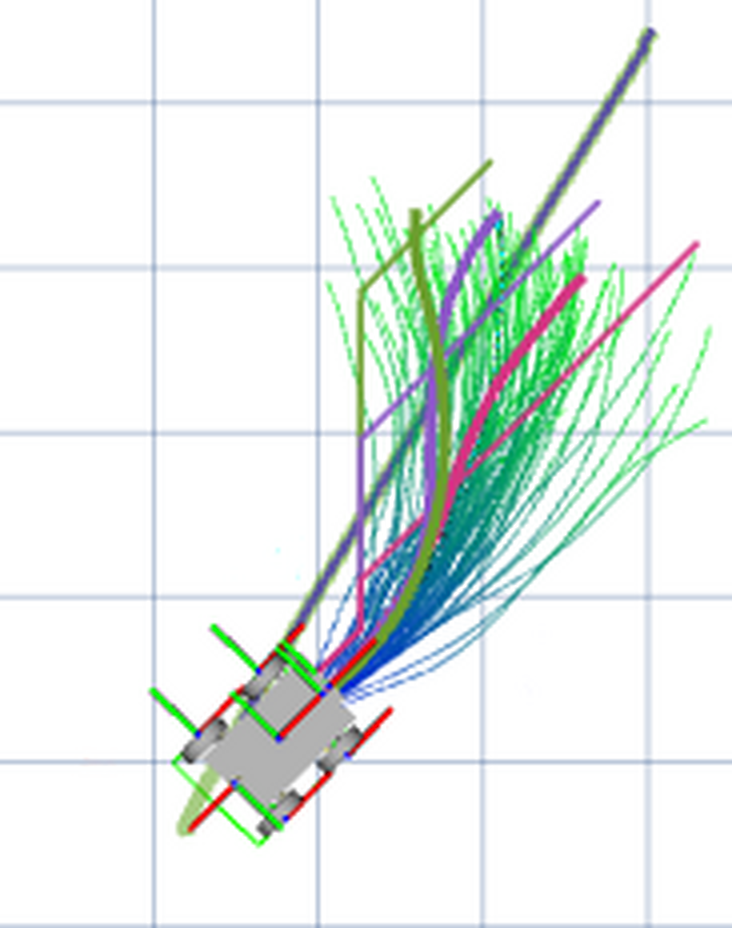
\includegraphics[width=0.48\columnwidth]{figures/multimodal_trajectory_motivation.png}
  \caption{Motivating snapshot of sampled MPPI rollouts (green), a nominal
  route (blue/grey), and pseudopod-derived guidance (magenta). The image
  illustrates route-conditioned sampling and is not a quantitative result.}
  \label{fig:trajectory-motivation}
\end{figure}

This problem is not only of academic interest for the platform targeted by
this work. SLIP -- Scalable Locomotion for Imperfect Places -- was built for
deployment on active construction sites, one of the clearest real-world
examples of an ``imperfect place'': stacked materials, parked machinery and
scaffolding create narrow passages that are reconfigured from day to day
rather than fixed like a warehouse floor plan, and workers and vehicles move
through them on timing the robot cannot control. The name also reflects a
second, everyday inspiration: dense, largely unregulated urban traffic of the
kind found on the roads of Chennai, India, where vehicles, pedestrians and
obstacles share the same narrow space with no reliable lane discipline or
predictable timing. Both settings are instances of the same underlying
class of environment. These are precisely the conditions under which a
single averaged MPPI route is expected to fail, not an adversarial edge case
constructed for a benchmark. Multimodal route preservation is therefore
treated in this work as a requirement of SLIP's intended deployment, not an
optional refinement of MPPI.

This work asks whether explicit local route modes improve MPPI beyond the
benefit obtained from predicting obstacle motion alone. To investigate this
question, TG-MPPI uses locally reachable topology to preserve multiple
candidate manoeuvres during sampling instead of collapsing them into a single
control distribution. Its behaviour is studied first in a controlled sandbox
and then through a matched Nav2/Gazebo comparison on a skid-steer robot.
The target is SLIP, a custom-built four-wheel skid-steer platform -- the same
drivetrain construction equipment uses for traction over uneven, debris-strewn
ground -- rather than an off-the-shelf differential-drive robot built for
structured indoor floors. Its geometry, sensing layout and velocity-command
interface impose the footprint and motion constraints used throughout this
work.

The contributions of this report are:
\begin{enumerate}
  \item an online method for deriving pseudopod-based ancillary controllers --
        candidate route trajectories traced from a local geodesic flood, one
        per distinct passable exit -- from locally reachable geodesic
        topology (Section~\ref{sec:method});
  \item a documented SLIP robot-to-simulation-to-Nav2 integration that makes
        the controller testable against the platform's geometry and sensing
        constraints (Section~\ref{sec:slip-platform});
  \item a scripted, reproducible dynamic-obstacle benchmark with ground-truth
        contact scoring, in which every condition sees identical obstacle
        trajectories (Section~\ref{sec:setup});
  \item an ablation separating the contribution of obstacle prediction from
        that of topological guidance (Section~\ref{sec:results}); and
  \item an evaluation of spatial and space--time guidance using a
        winding-based route-distinctness test (Section~\ref{sec:distinctness}).
\end{enumerate}

\section{Related Work}
Local motion planners for cluttered, dynamic environments broadly fall into
three families. Reactive geometric methods such as the Dynamic Window
Approach \cite{fox1997dwa} search directly over admissible instantaneous
velocities; they run cheaply and react immediately, but their short lookahead
makes them prone to local minima and to manoeuvres that only become unsafe a
few steps later. Gradient-based trajectory optimisers such as the Timed
Elastic Band \cite{roesmann2017teb} instead optimise a full short-horizon
trajectory against a smooth cost, giving better dynamic feasibility and
lookahead -- but a gradient descended from one initial guess converges to
whichever single local minimum it started nearest to. When the free space
around an obstacle is genuinely multimodal (pass left, pass right, wait), that
single-mode collapse is structural, not a tuning failure: the optimiser never
considers the alternative it did not start near.

Sampling-based stochastic control sidesteps that specific problem by
replacing the gradient with many randomly perturbed rollouts, reweighted by
their cost. MPPI casts finite-horizon stochastic control as such an
importance-weighted update over sampled control perturbations and maps
naturally to parallel hardware \cite{williams2017mppi,williams2018mppi}: it
evaluates complete short trajectories rather than admissible instantaneous
velocities or a single optimised one, so a good candidate through either side
of an obstacle can be discovered without a gradient ever pointing there. The
standard formulation nevertheless represents its solution with one nominal
sequence; it does not explicitly preserve multiple route classes when the
rollout distribution becomes multimodal -- the same collapse TEB suffers from
reappears one step later, at the reweighting stage instead of the gradient
step.

For mobile-robot control, MPPI is attractive because forward simulation can
accommodate nonlinear dynamics and non-convex combinations of path tracking,
goal progress, obstacle proximity, control effort and command variation without
requiring derivatives. This flexibility is not free: behaviour depends strongly
on horizon length, temperature, perturbation covariance, rollout-model fidelity
and the available sample budget. Longer horizons expose delayed collisions but
increase computation, while an uninformative proposal can spend most rollouts
on infeasible motion. These trade-offs are especially relevant to skid-steer
platforms, whose realised turning motion can depart from ideal unicycle
kinematics through lateral slip and wheel scrubbing
\cite{mandow2007skidsteer}. Receding-horizon replanning corrects new state
errors but does not by itself remove this model mismatch.

Existing MPPI variants address different parts of this practical problem.
Low-frequency perturbations introduce temporal correlation to reduce
high-frequency control variation \cite{vlahov2024lowfrequency}, while smooth
MPPI uses an input-lifting formulation to suppress command jitter without a
separate post-processing filter \cite{kim2022smooth}. Log-MPPI reshapes the
sampling distribution to improve exploration in clutter
\cite{mohamed2022logmppi}, and robust MPPI couples nominal sampling with
feedback reasoning under disturbances \cite{gandhi2021robust}. Closer to mode
preservation itself, SOPPI applies Stein Variational Gradient Descent (SVGD)
between MPPI steps so that a repulsive kernel force spreads sampled
trajectories apart and resists collapse onto a single mean
\cite{aldrich2025soppi}. That repulsion is generic and requires
differentiating the rollout through the cost and dynamics, which reintroduces
exactly the gradient fragility sampling-based MPPI was meant to avoid and has
so far only been demonstrated on cart-pole, arm and legged-locomotion
benchmarks rather than obstacle-cluttered navigation; it has no notion of
\emph{why} distinct modes exist in a particular scene. TG-MPPI instead derives
its modes directly from the locally reachable geodesic topology of the actual
environment, without differentiating anything. These methods
improve smoothness, exploration, execution robustness or generic sample
diversity, but none prescribes how to construct several environment-dependent
route modes and prevent their
control updates from cancelling one another.

Biased-MPPI generalises the sampling step by allowing ancillary controllers to
inject informative control sequences instead of drawing every candidate around
the shifted solution from the previous cycle \cite{trevisan2024biased}. This can
place samples near braking, tracking or learned strategies that ordinary local
Gaussian exploration might rarely discover. The ancillary controllers in that
work are supplied by the designer or a learned policy. TG-MPPI builds on this
idea but addresses a different question: how can the environment's currently
reachable topology generate those ancillary strategies online? Its pseudopods
and space--time routes answer that question, while grouped updates prevent
opposed strategies from being averaged together.

Topology-aware planners instead reason about families of paths that cannot be
continuously deformed into one another without crossing obstacles.
H-signatures provide a formal algebraic representation for search-based
planning \cite{bhattacharya2012hsignature}, while distinctive-topology TEB
optimises several elastic-band candidates online \cite{roesmann2017teb}. These
methods motivate keeping alternatives separate until their quality can be
compared, but they do not directly specify how a sampling-based controller
should construct and allocate its rollout distribution.

The closest methodological reference is topology-driven parallel trajectory
optimisation (T-MPC), which is explicitly presented by its authors as a
\emph{global} planner: a probabilistic-roadmap-style topology stage identifies
several distinct homotopy classes across the free space, and each seeds an
independent \emph{local} gradient-based optimiser running in parallel
\cite{degroot2025tmpc}. TG-MPPI adopts the same high-level
principle---preserve and compare distinct decisions---entirely inside the
local stage, for two reasons a global topology search would not fit. First,
Nav2 already supplies a global planner upstream of the controller
\cite{macenski2023nav2}; a second global topology stage inside the local
controller would duplicate that role rather than add to it. Second, T-MPC's
per-class cost is a full nonlinear program, so amortising it against a
global search is worthwhile; TG-MPPI's per-mode cost is instead a group of
sampled rollouts recomputed every control cycle regardless, so a cheap
rolling geodesic flood over the local costmap already gives the sampling
bias it needs without a separate global search. It represents the
alternatives as groups inside one MPPI rollout batch rather than as
independent gradient-based trajectory optimisers, and the result is packaged
within Nav2 as an unmodified Nav2 MPPI plugin standing in for the
operational baseline, rather than a separately reimplemented controller.

\section{Background and Problem Formulation}
\label{sec:problem}

\begin{table*}[t]
\centering
\caption{Notation. Symbols follow standard information-theoretic MPC usage
\cite{williams2017mppi,williams2018mppi,trevisan2024biased} where a
robotics-standard choice exists; problem-specific symbols are defined once,
here and at first use, and are not reused for anything else in this paper.}
\label{tab:notation}
\begin{tabular}{cl@{\hspace{2.2em}}cl}
\toprule
Symbol & Meaning & Symbol & Meaning \\
\midrule
$\mathbf x_t,\ \mathbf u_t$ & Robot state, control at step $t$ &
  $\mathcal B_\rho$ & Geodesic flood body ($\rho$-sublevel set of $d_r$) \\
$U=(\mathbf u_0,\ldots,\mathbf u_{T-1})$ & Control sequence over the horizon &
  $\partial\mathcal B_\rho$ & Outward flood membrane \\
$S(U)$ & Trajectory cost, Eq.~\eqref{eq:trajectory-cost} &
  $\operatorname{Adj}_8(p)$ & 8-connected grid neighbours of $p$ \\
$P,\ Q$ & Reference / optimised control distributions &
  $h(m)$ & Terminal cost-to-go (``promise'') at membrane cell $m$ \\
$\lambda$ & MPPI temperature (cost/KL trade-off) &
  $\eta(p)$ & Narrow-channel obstacle-proximity weight \\
$w^{(i)}$ & Self-normalised sample weight &
  $D_g(p)$ & Weighted navigation value inside the body \\
$q_s(U)$ & Ancillary (biased) sampling proposal density &
  $P_m$ & Topology-distinct branch (pseudopod) centreline \\
$\pi_m,\ \boldsymbol\mu_m,\ \Sigma_m$ & Weight, mean, covariance of ancillary mode $m$ &
  $\boldsymbol\mu_m$ & Ancillary control-sequence mean from branch $P_m$, Eq.~\eqref{eq:ancillary-short} \\
$\Delta r$ & Local costmap / flood grid resolution &
  $\mathcal G_g,\ F_g$ & Sample group $g$ and its free energy \\
$r_p$ & Circular planning-footprint radius &
  $\hat o_j(\tau_k)$ & Predicted position of obstacle $j$ at time $\tau_k$ \\
$d_r(p)$ & Geodesic (obstacle-free) distance from the robot to $p$ &
  $\lambda_{\mathrm w}$ & Normalised winding number, Eq.~\eqref{eq:winding} \\
$\mathcal F$ & Collision-free grid cells &
  $\rho$ & Geodesic flood reach (a travel-distance budget) \\
\bottomrule
\end{tabular}
\end{table*}

\subsection{Information-theoretic stochastic control}
Consider a robot with state $\mathbf{x}_t\in\mathbb R^n$ and control
$\mathbf{u}_t\in\mathbb R^m$ evolving under
$\mathbf{x}_{t+1}=f(\mathbf{x}_t,\mathbf{u}_t)$. For the horizon control
sequence $U=(\mathbf u_0,\ldots,\mathbf u_{T-1})$, define
\begin{equation}
 S(U)=\phi(\mathbf x_T)+\sum_{t=0}^{T-1}
 \ell(\mathbf x_t,\mathbf u_t),
 \label{eq:trajectory-cost}
\end{equation}
where $S$ may include goal, path, constraint, static-obstacle and predicted
dynamic-obstacle terms. Let $P$ be a reference distribution over control
sequences. The information-theoretic formulation seeks a distribution $Q$
that minimises
\begin{equation}
 \mathcal J(Q)=\mathbb E_Q[S(U)]+\lambda D_{\mathrm{KL}}(Q\Vert P),
 \label{eq:free-energy-objective}
\end{equation}
where $\lambda>0$ trades expected trajectory cost against departure from $P$.

Introducing a multiplier for $\int q(U)dU=1$ and setting the functional
derivative of~\eqref{eq:free-energy-objective} to zero yields
\begin{align}
 0&=S(U)+\lambda\left[\log\frac{q^*(U)}{p(U)}+1\right]+\beta,\\
 q^*(U)&=\frac{1}{\eta}\exp\!\left[-\frac{S(U)}{\lambda}\right]p(U),
 \label{eq:optimal-control-distribution}\\
 \eta&=\mathbb E_P\!\left[\exp\!\left(-\frac{S(U)}{\lambda}\right)\right].
\end{align}
Low-cost sequences therefore receive exponentially greater probability, while
$\lambda$ determines how sharply the distribution concentrates.

\subsection{Classical MPPI}
Classical MPPI samples $N$ sequences
$U^{(i)}=\bar U+\mathcal E^{(i)}$ around the shifted solution from the previous
cycle and rolls each sequence through the dynamics. With the standard MPPI
trajectory cost, including its control/noise term, the Monte-Carlo update is
\begin{align}
  w^{(i)}
  &=\frac{\exp[-(S^{(i)}-S_{\min})/\lambda]}
          {\sum_{j=1}^{N}\exp[-(S^{(j)}-S_{\min})/\lambda]},\\
  \mathbf{u}^{*}_t
  &=\bar{\mathbf u}_t+
    \sum_{i=1}^{N} w^{(i)}\boldsymbol\epsilon^{(i)}_t .
  \label{eq:mppi}
\end{align}
Subtracting $S_{\min}$ is numerically stabilising and does not alter the
normalised weights. The first updated command is applied, the remaining
sequence is shifted forward, and the calculation repeats at the next cycle
\cite{williams2017mppi,williams2018mppi}.

\subsection{Biased MPPI and ancillary controllers}
The shifted previous solution is useful when the scene changes slowly, but it
can concentrate the entire sample population around a newly invalid strategy.
Biased-MPPI permits an alternative sampling distribution $Q_s$ informed by
ancillary controllers \cite{trevisan2024biased}. For samples
$U^{(i)}\sim q_s$, the general importance-sampling form is
\begin{align}
 \widetilde w^{(i)}
 &=\exp\!\left[-\frac{S(U^{(i)})}{\lambda}\right]
   \frac{p(U^{(i)})}{q_s(U^{(i)})},
 \label{eq:biased-mppi-weight}\\
 w^{(i)}&=\frac{\widetilde w^{(i)}}{\sum_j\widetilde w^{(j)}},
 \qquad
 \mathbf u_t^*\approx\sum_iw^{(i)}\mathbf u_t^{(i)}.
 \label{eq:biased-mppi-update}
\end{align}
The density ratio corrects for drawing from $Q_s$ rather than $P$; equivalently,
its logarithm can be absorbed into an augmented trajectory cost. For $M$
ancillary controllers producing horizon-length means $\mu_m$, the proposal can
be represented as
\begin{equation}
 q_s(U)=\sum_{m=0}^{M}\pi_m
 \mathcal N(U;\mu_m,\Sigma_m),\qquad \sum_m\pi_m=1,
 \label{eq:biased-mixture}
\end{equation}
where $m=0$ is the nominal or global-path fallback. Biased-MPPI supplies the
mechanism for injecting and fusing ancillary strategies, but it does not
prescribe that their means must represent locally distinct collision-free
routes. TG-MPPI's contribution begins there: it generates $\mu_m$ online from
geodesic pseudopods and space--time alternatives.

For clarity, the sandbox includes the explicit density correction
of~\eqref{eq:biased-mppi-weight}, but the evaluated Nav2 controller uses the
conditional within-group softmax estimator of~\eqref{eq:grouped-objective}
(implementation details in Section~\ref{sec:impl}): costs are normalised
within each proposal group and the minimum-free-energy group's weighted
update is applied, without correcting for the fact that the samples were
drawn from a mixture proposal. It inherits Biased-MPPI's ancillary-proposal
principle, but is not claimed to be an exact implementation of its
fully importance-corrected estimator.

\subsection{Multimodal failure addressed by TG-MPPI}
Equation~\eqref{eq:mppi} still forms one control average. If similarly weighted
samples pass an obstacle on opposite sides, their average can lie between the
two modes and commit to neither. Let $\mathcal O_{0:T}$ denote the static and
predicted dynamic obstacle set. Two feasible trajectories $\xi_a$ and $\xi_b$
are in the same space--time homotopy class when one can be continuously
deformed into the other without intersecting $\mathcal O_{0:T}$ while their
endpoints remain fixed. Partitioning samples into candidate classes
$\mathcal G_g$ changes the decision into a conditional update followed by
explicit selection,
\begin{equation}
  g^*=\arg\min_g F_g, \qquad
  \mathbf u_t^*=\sum_{i\in\mathcal G_{g^*}}w_{i\mid g^*}
  \mathbf u_t^{(i)} .
  \label{eq:grouped-objective}
\end{equation}
The objective is not to prove that every possible class has been enumerated,
but to preserve a small set of useful local decisions long enough for MPPI to
compare them without averaging opposed controls together.

\section{Method: TG-MPPI}
\label{sec:method}
Figure~\ref{fig:pipeline} summarises the complete receding-horizon computation.
The first stage is the proposed topology-to-ancillary-controller construction;
the second and third stages evaluate and commit to one proposal without
averaging across opposed route modes.

\begin{figure*}[t]
  \centering
  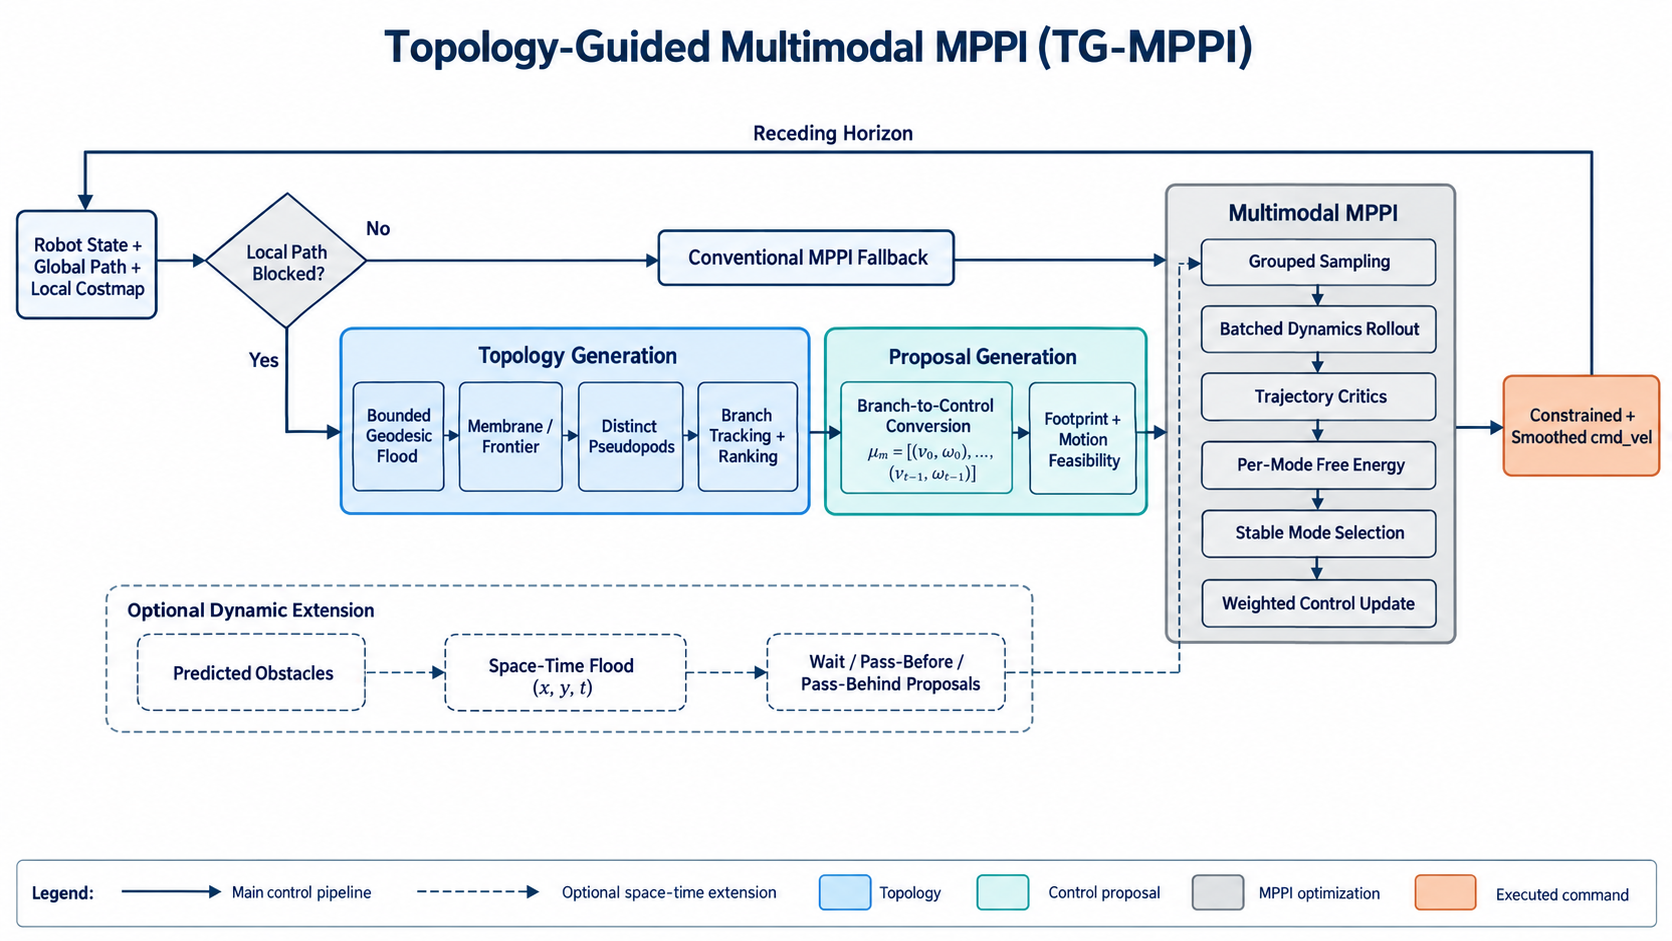
\includegraphics[width=0.96\textwidth]{figures/tg_mppi_flowchart.png}
  \caption{TG-MPPI architecture. Robot state, local geometry, the Nav2 global
  path and predicted obstacle motion generate collision-validated spatial and
  space--time ancillary means. Separate MPPI sample groups are rolled out and
  scored by the common critic set. A committed-mode decision selects one
  conditional update, whose first command is executed before replanning.}
  \label{fig:pipeline}
\end{figure*}

\subsection{Geodesic flood field and the robot-centred body}
The local costmap is discretised at resolution $\Delta r$ and obstacles are
inflated by a circular planning-footprint radius $r_p$. The remaining free
cells form an eight-connected graph, with axial edge cost $\Delta r$ and
diagonal cost $\sqrt{2}\Delta r$. A single-source Dijkstra expansion from the
robot gives the collision-free geodesic distance
\begin{equation}
 d_r(p)=\min_{\gamma:p_r\leadsto p}\sum_{e\in\gamma}w(e).
 \label{eq:local-geodesic}
\end{equation}
Dijkstra is used instead of A* because the distances to all reachable cells,
not one known endpoint, are required. The geodesic body is the sublevel set
\begin{equation}
 \mathcal B_\rho(p_r)=\{p\in\mathcal F:d_r(p)\leq\rho\},
 \label{eq:geodesic-body}
\end{equation}
where $\rho$ is a travel-distance budget rather than a Euclidean radius. It is
approximately circular in open space, but deforms around inflated obstacles
and pinches through connected passages. The body is rebuilt from the current
robot pose at the configured field-update rate; it is therefore a rolling
reachability construction, not a fixed shape translated through the map.

Its outward membrane contains body cells adjacent to reachable free space just
beyond the budget,
\begin{equation}
 \partial\mathcal B_\rho=\{p\in\mathcal B_\rho:\exists q\in
 \operatorname{Adj}_8(p),\ q\in\mathcal F\setminus\mathcal B_\rho\}.
 \label{eq:membrane-short}
\end{equation}
A wall-facing body edge is consequently not treated as a possible exit merely
because it borders an obstacle.

Figure~\ref{fig:amoeba-motion} shows three rebuilds produced by the actual
Python sandbox in BARN world 48. The changing outline illustrates the key
geodesic property: the body measures connected travel through free space and
therefore changes shape rather than translating as a rigid Euclidean disc.

\begin{figure*}[t]
  \centering
  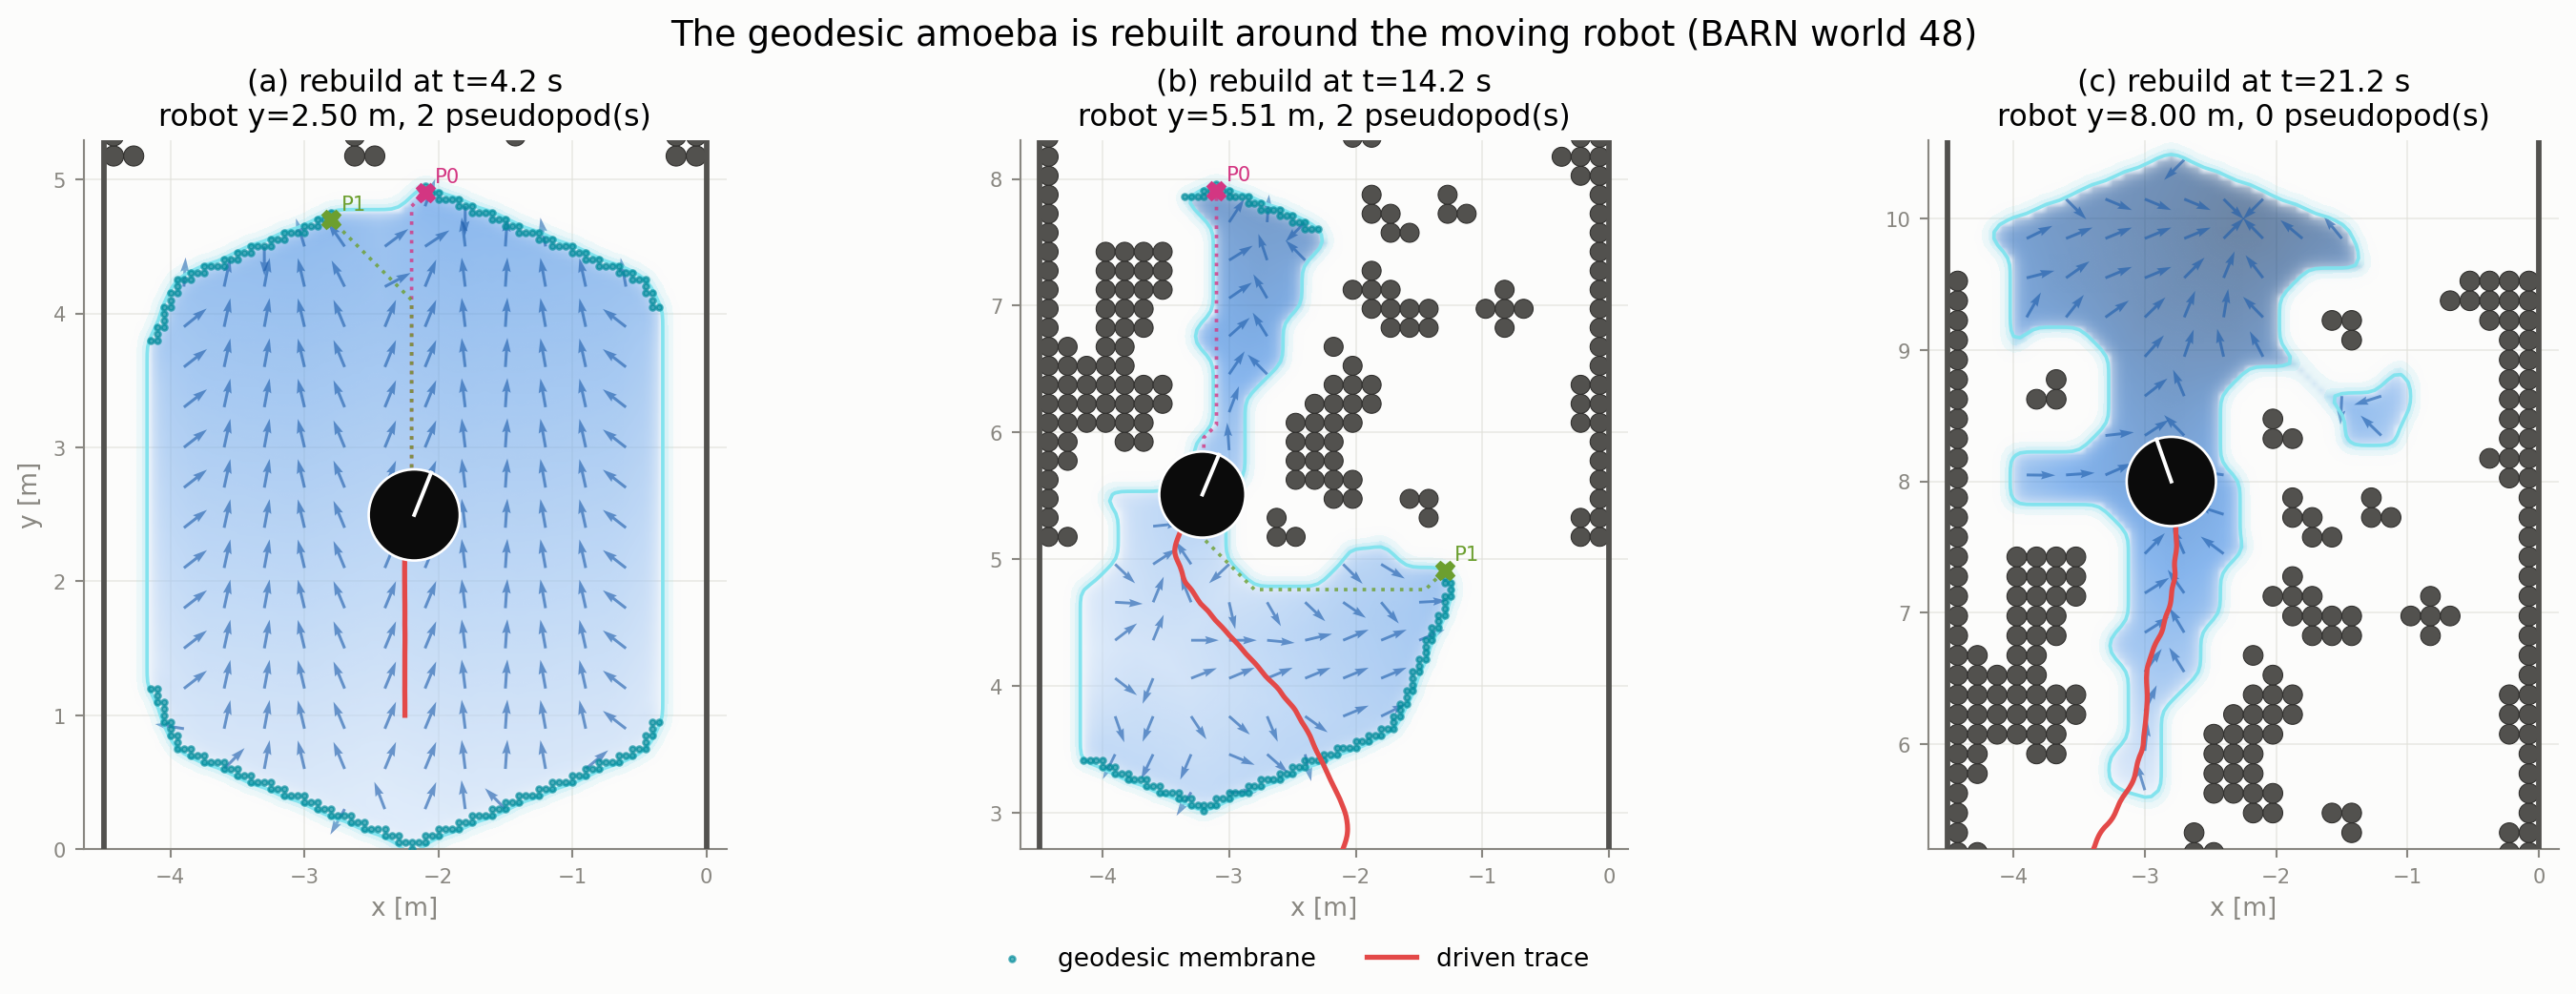
\includegraphics[width=\textwidth]{../../artifacts/images/demos/amoeba_motion_sequence.png}
  \caption{Sandbox execution in BARN world 48. The geodesic body (blue),
  membrane (cyan), navigation directions (arrows), retained pseudopods
  (dotted curves) and driven trace (red) are shown at three field rebuilds.
  This is an implementation-derived explanatory visual, not a scored Nav2
  benchmark trial.}
  \label{fig:amoeba-motion}
\end{figure*}

\subsection{Pseudopod branches as guidance trajectories}
A \emph{pseudopod} is, concretely, a single traced path from one promising
membrane exit back to the robot, converted into one ancillary control
sequence -- the name borrows the biological term for a temporary protrusion
an amoeba extends toward a direction it may move in, since the flood body
here does the same thing toward each candidate route before the robot
commits to one. The previous section built one geodesic distance field per
cycle; this section selects a handful of its membrane cells as pseudopod
endpoints and turns each into an ancillary mean trajectory a sample group can
be centred on. Every membrane cell $m$ first receives a terminal cost-to-go,
or \emph{promise},
from the global path $\mathcal P=\{z_k\}$,
\begin{equation}
 h(m)=\min_{z_k\in\mathcal P}
 \left(\lVert m-z_k\rVert_2+L_{\mathrm{rem}}(z_k)\right),
 \label{eq:promise-short}
\end{equation}
where $L_{\mathrm{rem}}$ is remaining path arclength. The name is heuristic:
$h$ is neither a probability nor a guarantee. A second multi-source Dijkstra
field propagates these boundary values inward with an obstacle-proximity
penalty $\eta(p)$,
\begin{equation}
 D_g(p)=\min_{m\in\partial\mathcal B_\rho}
 \left[h(m)+d_\eta(p,m)\right],
 \label{eq:navigation-short}
\end{equation}
so narrow, low-clearance channels remain reachable but are less attractive.

Candidate endpoints are ranked by $D_g(m)+d_r(m)$ and spatially suppressed to
remove nearby duplicates. Each retained endpoint is traced back to the robot by
descending $d_r$. A connector test rejects branches that are geometrically
separated at their endpoints but not separated by an obstacle; at most three
local branches are retained and tracked between field rebuilds. For branch
$P_m$, a branch-following policy produces a horizon-length ancillary mean
\begin{equation}
 \boldsymbol\mu_m=\mathcal A(P_m,x_0)
   =[\mathbf u_{m,0},\ldots,\mathbf u_{m,T-1}],
 \label{eq:ancillary-short}
\end{equation}
subject to velocity and acceleration limits. Its full rectangular-footprint
rollout is collision-checked before it may seed a proposal group.

\subsection{Grouped sampling and per-group free energy}
Rather than running an independent optimiser per homotopy class, TG-MPPI
partitions a single rollout batch into groups, one per active guidance mode plus
a fallback group warm-started from the previous solution. Each group $g$ is
warm-started from its own guidance trajectory and scored by its own free energy
\begin{equation}
  F_g = c^{\min}_g - \lambda \log \frac{1}{|g|}\sum_{i \in g}
        \exp\!\left(-\tfrac{1}{\lambda}\left(S^{(i)} - c^{\min}_g\right)\right),
  \label{eq:freeenergy}
\end{equation}
and the group with the lowest $F_g$ is selected, with a switch margin to
suppress chattering.

A consequence of~\eqref{eq:freeenergy} deserves note: $c^{\min}_g$ is a minimum
over $|g|$ samples, so its expectation decreases with group size roughly as
$-\sigma\sqrt{2\ln|g|}$. A large fallback group therefore enjoys a systematic
head start over small guidance groups, independent of trajectory quality. Both
an unequal (\emph{legacy}) and an equal-share allocation are evaluated in
Section~\ref{sec:results}.

Algorithm~\ref{alg:tgmppi} states the complete online procedure. Operations up
to branch generation run at the lower flood-field update rate; sampling,
rollout, scoring and selection run every control cycle.

\begin{algorithm}[t]
\caption{Topology-Guided Grouped MPPI}
\label{alg:tgmppi}
\begin{algorithmic}[1]
\Require state $x_k$, costmap $C_k$, path $\mathcal P$, tracked obstacles
$\hat{\mathcal O}_{0:T}$, batch $N$, horizon $T$
\Ensure applied control $u_k^*$
\State $\mathcal F\gets\Call{InflatedFreeCells}{C_k,r_p}$
\State $d_r\gets\Call{Dijkstra}{p_k,\mathcal F}$
\State $\mathcal B_\rho\gets\{p\in\mathcal F:d_r(p)\leq\rho\}$
\State $\partial\mathcal B_\rho\gets\Call{OutwardBoundary}{\mathcal B_\rho,\mathcal F}$
\State $D_g\gets\Call{NavigationField}{\partial\mathcal B_\rho,\mathcal P,C_k}$
\State $\{P_m\}\gets\Call{DistinctBacktraces}{d_r,D_g,\mathcal F}$
\State $\{P_m\}\gets\{P_m\}\cup
\Call{STAlternatives}{\{P_m\},\hat{\mathcal O}_{0:T}}$
\State $\mathcal M\gets\{\Call{ProjectValid}{P_m,x_k,T,C_k}\}$
\State discard infeasible means; add nominal/path fallback $\mu_0$
\State $\{N_m\}\gets\Call{AllocateGroups}{N,\mathcal M}$
\ForAll{$m\in\mathcal M$}
  \State $U_m^{(i)}\sim\mathcal N(\mu_m,\Sigma_m)$, $i=1,\ldots,N_m$
  \State $X_m^{(i)}\gets\Call{Rollout}{x_k,U_m^{(i)}}$
  \State $S_m^{(i)}\gets\Call{Nav2Critics}{X_m^{(i)},U_m^{(i)},\hat{\mathcal O}_{0:T}}$
  \State $(F_m,w_{i\mid m},\bar U_m)\gets\Call{ConditionalUpdate}{S_m,U_m}$
\EndFor
\State $m^*\gets\Call{CommitMode}{\{F_m\},\text{dwell, margin, confirm}}$
\State $u_k^*\gets(\bar U_{m^*})_0$
\State \Return $u_k^*$
\end{algorithmic}
\end{algorithm}

\subsection{Space-time routes}
Spatial pseudopods distinguish routes around static geometry but cannot encode
that the same position may be blocked at one arrival time and free at another.
TG-MPPI therefore constructs a coarser time-expanded graph whose vertices are
$(p,k)$, with $\tau_k=k\Delta t_\ell$. Every transition advances one time
layer and either moves to an eight-connected neighbour or waits in place. For
constant-velocity obstacle prediction
\begin{equation}
 \hat o_j(\tau_k)=o_j+v_j\min(\tau_k,T_{\mathrm{pred}}),
 \label{eq:cv-prediction}
\end{equation}
a space--time vertex is free only when both the static footprint constraint and
\begin{equation}
 \lVert p-\hat o_j(\tau_k)\rVert_2>r_p+r_j
 \quad\forall j
 \label{eq:spacetime-free-short}
\end{equation}
hold. Diagonal moves additionally forbid corner cutting.

Dijkstra search is run twice with different costs for the wait transition. A
low wait cost favours yielding until the crossing clears; a high wait cost
favours continued motion and hence a spatial detour. This produces candidate
routes $\pi_{\mathrm{wait}}$ and $\pi_{\mathrm{detour}}$, which are converted
to ancillary control means by the same constrained branch-following procedure
as the spatial pseudopods. The search is proposal generation, not collision
avoidance by itself: the predicted-obstacle critic still scores every MPPI
rollout. Only routes that pass the winding-based distinctness test below are
added as separate groups.

The space--time proposal subroutine is given in
Algorithm~\ref{alg:spacetime}. Running the graph search with two wait costs is
what creates a timing alternative; the winding test decides whether it adds a
meaningfully different mode.

\begin{algorithm}[t]
\caption{Space--Time Alternative Generation}
\label{alg:spacetime}
\begin{algorithmic}[1]
\Require pseudopods $\{P_m\}$, predicted obstacles $\hat{\mathcal O}_{0:T_s}$
\Ensure distinct wait/detour candidates $\mathcal A_{st}$
\State $\mathcal A_{st}\gets\varnothing$
\ForAll{$P_m$ in priority order}
  \State $o^*\gets\Call{NearestPredictedCrossing}{P_m,\hat{\mathcal O}_{0:T_s}}$
  \If{$o^*$ exists}
    \State $G_{st}\gets\Call{TimeGraph}{P_m,o^*,\Delta r_s,\Delta t_\ell}$
    \State $\pi_w\gets\Call{Dijkstra}{G_{st},c_w^{\mathrm{cheap}}}$
    \State $\pi_d\gets\Call{Dijkstra}{G_{st},c_w^{\mathrm{expensive}}}$
    \ForAll{$\pi\in\{\pi_w,\pi_d\}$}
      \State $\mu_\pi\gets\Call{ProjectValid}{\pi,x_k,T,C_k}$
      \If{$\mu_\pi$ feasible and \Call{OppositeWinding}{$\pi,P_m,o^*$}}
        \State $\mathcal A_{st}\gets\mathcal A_{st}\cup\{\pi\}$
      \EndIf
    \EndFor
    \State \textbf{break} \Comment{bounded single-crossing budget}
  \EndIf
\EndFor
\State \Return $\mathcal A_{st}$
\end{algorithmic}
\end{algorithm}

Figure~\ref{fig:spacetime-topology} visualises the construction in both the
ground plane and the time-expanded volume. A moving obstacle becomes a tube in
$(x,y,t)$; waiting and detouring pass different sides of that tube even when
their two-dimensional projections partially overlap.

\begin{figure*}[t]
  \centering
  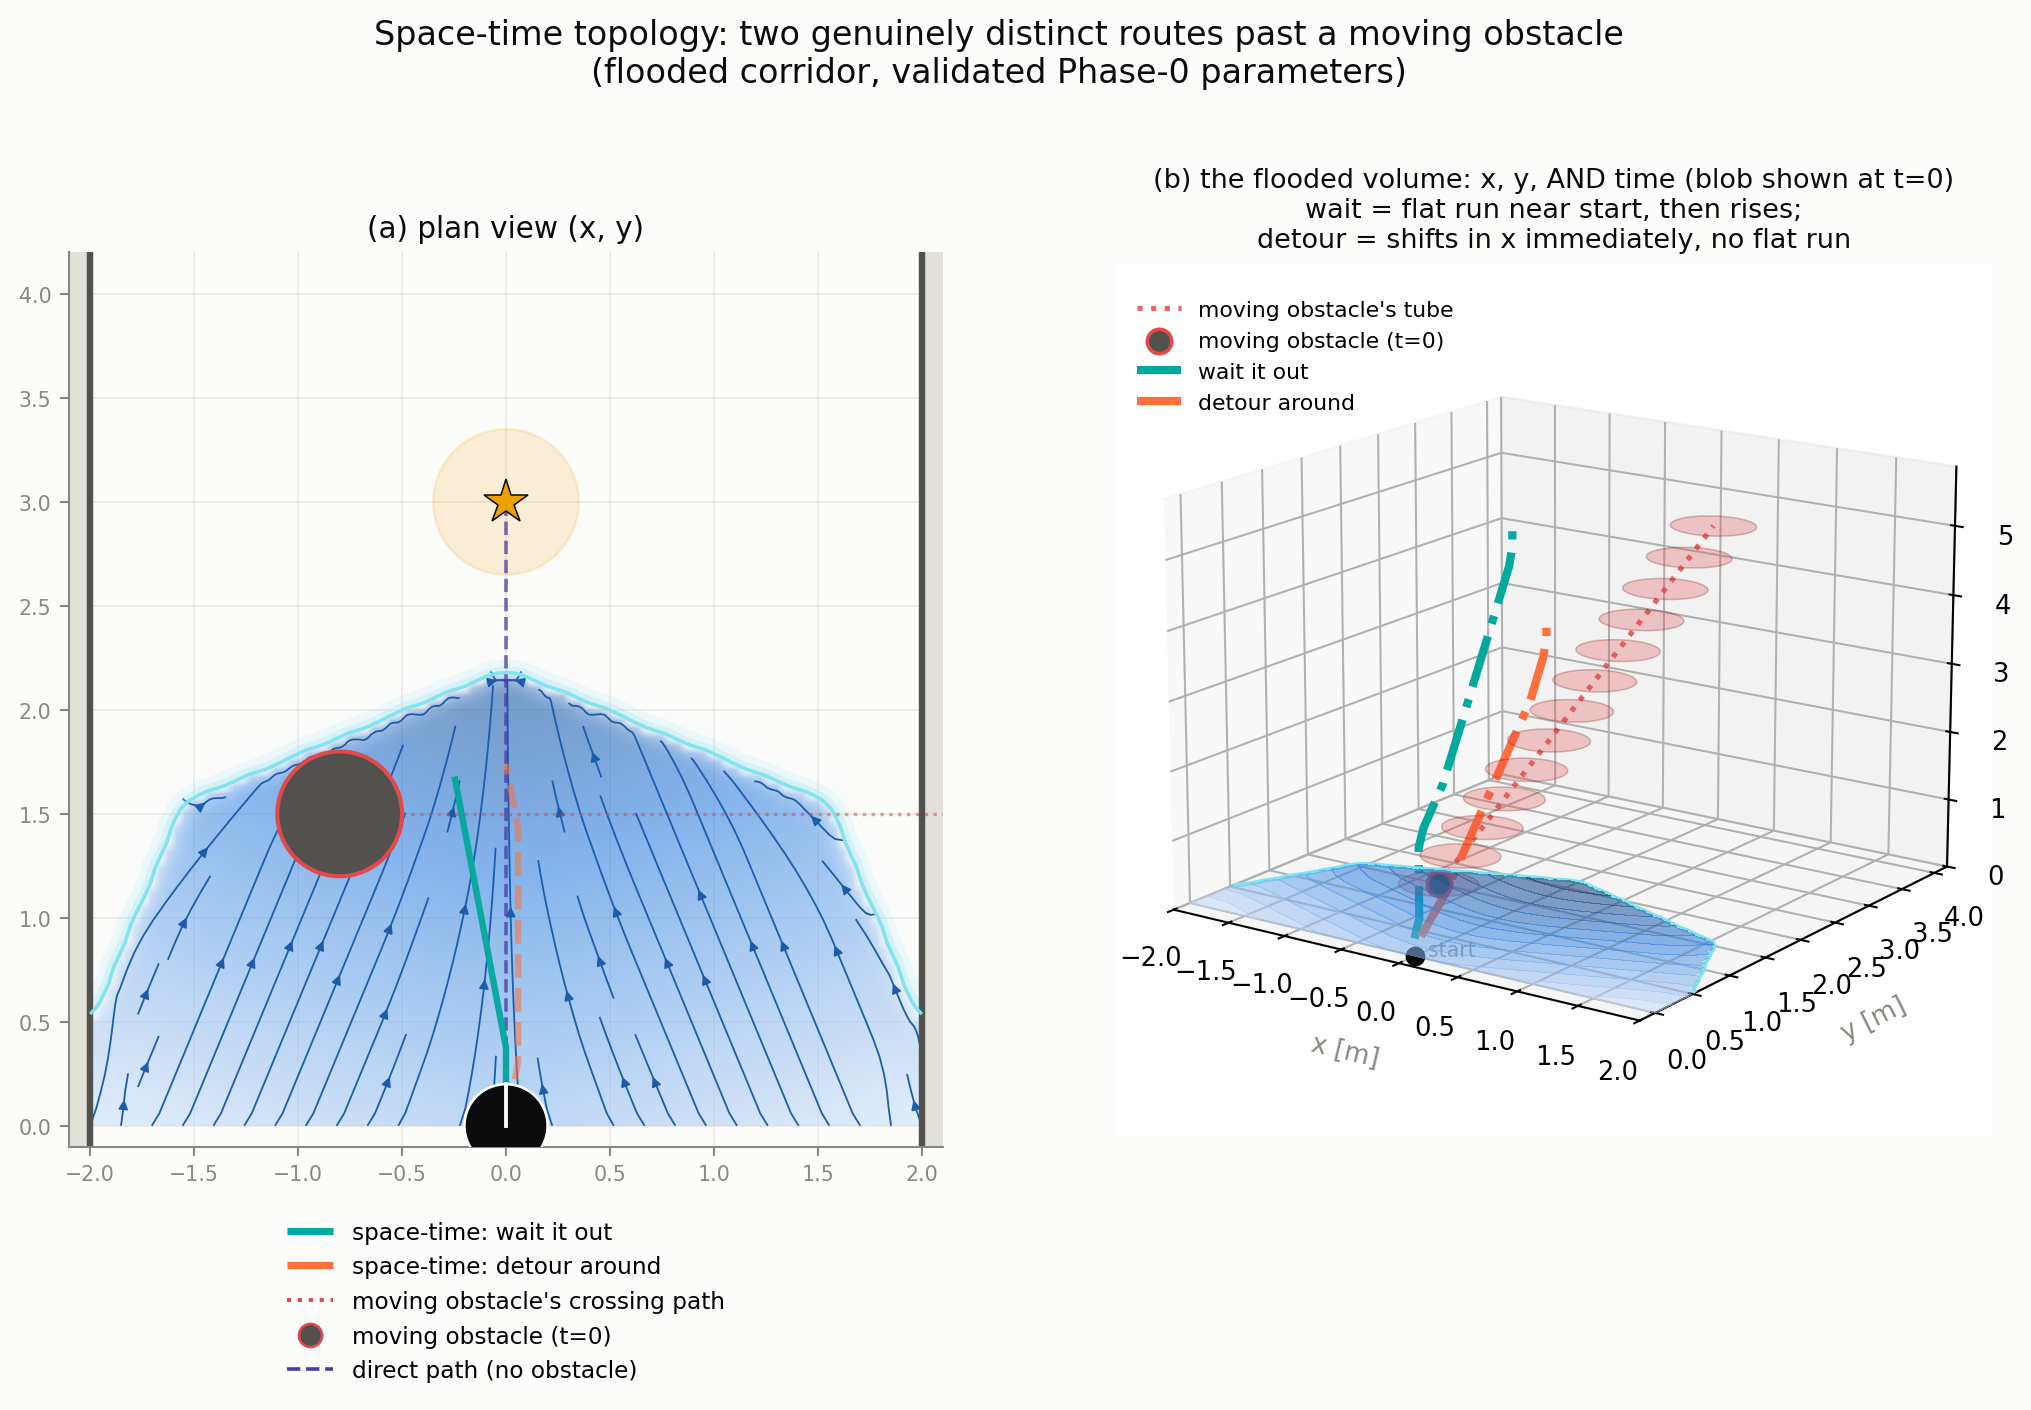
\includegraphics[width=0.76\textwidth]{../../artifacts/images/demos/spacetime_topology.png}
  \caption{Synthetic sandbox demonstration of space--time topology. Left:
  plan view of wait and detour candidates around a moving obstacle. Right:
  the same candidates in $(x,y,t)$, where the obstacle trajectory forms an
  exclusion tube. The diagram explains the proposal mechanism; quantitative
  claims are drawn only from the Gazebo benchmark.}
  \label{fig:spacetime-topology}
\end{figure*}

\subsection{Homotopy distinctness}
\label{sec:method-distinct}
Two candidate routes are only worth optimising separately if they are
homotopically distinct. Let $\mathbf{p}(t)$ be a route and $\mathbf{o}(t)$ the
predicted position of an obstacle. The normalised winding number
\begin{equation}
  \lambda_{\mathrm{w}} = \frac{1}{2\pi}\sum_{k=1}^{K}
      \operatorname{wrap}\!\big(\theta_k - \theta_{k-1}\big),
  \qquad
  \theta_k = \operatorname{atan2}\!\big(\mathbf{p}_k - \mathbf{o}_k\big),
  \label{eq:winding}
\end{equation}
accumulates the relative angle over the whole route, where
$\operatorname{wrap}(\cdot)$ maps to $(-\pi,\pi]$. A route is taken to have
passed the obstacle when $|\lambda_{\mathrm{w}}| \ge 1/(4\pi)$, and two routes
are distinct when both pass it with opposite sign. This follows the winding-number
test of T-MPC \cite{degroot2025tmpc}, which reports it as statistically
equivalent to an H-signature \cite{bhattacharya2012hsignature} at lower cost.

Section~\ref{sec:distinctness} reports why an earlier synchronised-time
side test, which required both routes to be near the same obstacle at the same
time step, was structurally unable to detect the distinction it existed to test.

\section{Implementation}
\label{sec:impl}
TG-MPPI is implemented as a \texttt{nav2\_core::Controller} plugin for ROS~2
Humble, loadable in place of the stock \texttt{nav2\_mppi\_controller}. The
baseline is the unmodified upstream controller; no change was made to it at any
point, so baseline and treatment differ only in the plugin selected at launch.

The controller runs at \SI{20}{Hz} with $N=2000$ samples, $T=56$ steps, and
$\Delta t={}$\SI{0.05}{s}. Its critic chain contains the stock constraint,
costmap, goal, goal-angle, path-align, path-follow, path-angle and
prefer-forward terms, augmented by the predicted-obstacle critic. The flow
critic is loaded but disabled in the reported configuration, isolating the
effect of ancillary sampling. Rollout and the supported critic operations use
a LibTorch/CUDA backend; unsupported operations retain a CPU path and the
controller falls back to CPU if CUDA is unavailable. The control-period budget
is \SI{50}{ms}.

The Nav2 implementation uses within-group (conditional) softmax weighting
rather than full-mixture importance correction: costs are normalised
within each proposal group, group free energies are compared, and only the
selected group's weighted control update is applied. Dwell time, a free-energy
switch margin, confirmation cycles and per-mode warm starts suppress mode
chattering. It does \emph{not} apply the explicit proposal-density correction
$\log p(U)-\log q(U)$ of full importance-corrected Biased MPPI. Consequently,
the thesis evaluates a topology-guided grouped MPPI implementation, while the
importance-corrected estimator remains a sandbox formulation rather than a
claim about the deployed Nav2 controller.

\subsection{SLIP platform and digital representation}
\label{sec:slip-platform}
SLIP was built as a four-wheel skid-steer mobile robot for navigation in
constrained spaces, with active construction sites as the primary intended
deployment setting: narrow, temporary passages between stacked materials and
equipment, and worker/vehicle traffic on timing the robot cannot control,
motivate the topological guidance problem studied in this report. The project
includes a CAD-derived ROS robot description
with the chassis, four wheel joints, sensor frames and collision geometry, and
a Gazebo model using the same frame layout. The wheel joints have no steering
degree of freedom: changes in heading require differential wheel-side speeds
and tyre--ground scrubbing. This matters because a commanded angular velocity
does not uniquely determine the realised turn on the physical platform.

The navigation interface accepts the same planar linear/angular velocity
(\texttt{cmd\_vel}) commands a differential-drive robot would: the control
stack is unaware that the platform is mechanically skid-steer. Skid-steer
behaviour is realised entirely below this interface, by the wheel-side speed
mixer and tyre--ground scrubbing described above; the planner and controller
both reason in the same unicycle-like command space regardless of the true
mechanism, which is itself a source of plant/model mismatch this report
returns to in Section~\ref{sec:discussion}.
The simulation drive plugin maps these commands to the wheel pairs using a
\SI{0.74}{m} track width and \SI{0.33}{m} wheel diameter. Local planning uses a
\SI{0.84}{m}$\times$\SI{0.68}{m} rectangular footprint rather than a point or
circular robot. The robot description locates front and rear lidar frames, an
IMU and a depth-camera frame; the benchmark costmap consumes front and rear
laser observations as separate sources. The dynamic benchmark uses the
simulated lidars and a ground-truth map pose, whereas the planned physical
trial will use the onboard lidar and Vicon. Those sources must not be treated
as equivalent evidence of perception or localisation robustness.

This platform work is an engineering contribution: constructing a robot and
its consistent digital/navigation interfaces makes controller transfer
possible. It is not presented as proof of a new skid-steer mechanism or a
validated slip model. The present quantitative claims come from sandbox and
Gazebo experiments; hardware tracking error, latency, slip and safety remain
to be measured in the physical validation study.

\subsection{Development sandbox and transfer to Nav2}
The algorithm was first developed in an independent NumPy/PyTorch sandbox. It
provides deterministic BARN-map loading, ideal and analytical-slip motion
models, A* references, geodesic-body and pseudopod extraction, grouped MPPI,
dynamic-obstacle prediction, space--time search, visualisation and ablation
harnesses. This environment was used to inspect algorithmic mechanisms and to
reject unsafe or ineffective variants before integration.

The sandbox and Nav2 controller are not treated as interchangeable
implementations. The final quantitative comparison uses the C++
\texttt{nav2\_tgmppi\_controller} plugin in Gazebo, with the same Nav2 lifecycle,
costmaps, global plans and robot interfaces as the stock baseline. Sandbox
results support design decisions and explanatory figures such as
Fig.~\ref{fig:amoeba-motion}; they are not pooled with Gazebo trials in the
headline statistics.

\section{Experimental Setup}
\label{sec:setup}

\subsection{Robot and simulator}
Experiments use the SLIP model described in Section~\ref{sec:slip-platform}
with Gazebo Classic 11 and ROS~2 Humble. The benchmark launch sets
$v_{x,\max}={}$\SI{1.5}{\metre\per\second}; the controller additionally enforces
its configured acceleration and yaw-rate limits. Planning and contact scoring
use the rectangular footprint. Localisation is supplied from Gazebo ground
truth through the map--odometry interface intended for motion-capture
localisation on the physical platform; AMCL is therefore not part of the
reported comparison.

\begin{table}[t]
\centering
\caption{System parameters used in the reported Nav2/Gazebo experiments
(Table~\ref{tab:main}, \ref{tab:blob}), read from the deployed controller
configuration. Values that vary by design across an experiment (e.g.\
$v_{x,\max}$ under the dynamic-obstacle command-speed override, described in
Section~\ref{sec:setup}) are reported there instead of here.}
\label{tab:params}
\begin{tabular}{lll}
\toprule
Parameter & Symbol & Value \\
\midrule
\multicolumn{3}{l}{\textit{Sampling}} \\
Samples per cycle & $N$ & 2000 \\
Horizon length & $T$ & 56 steps \\
Control/model time step & $\Delta t$ & \SI{0.05}{\second} \\
MPPI temperature & $\lambda$ & 0.3 \\
\addlinespace
\multicolumn{3}{l}{\textit{Geodesic body and pseudopods}} \\
Grid / costmap resolution & $\Delta r$ & \SI{0.025}{\metre} \\
Flood reach (travel-distance budget) & $\rho$ & \SI{2.5}{\metre} \\
Flood re-flood interval & --- & every control cycle \\
Retained branches (pseudopods) & --- & 3 \\
Branch match distance (re-identification) & --- & \SI{1.0}{\metre} \\
\addlinespace
\multicolumn{3}{l}{\textit{Mode selection}} \\
Free-energy switch margin & --- & 0.3 \\
Minimum dwell before a switch & --- & 10 cycles \\
Switch confirmation window & --- & 3 cycles \\
\addlinespace
\multicolumn{3}{l}{\textit{Robot}} \\
Footprint (length $\times$ width) & --- & \SI{0.84}{m}$\times$\SI{0.68}{m} \\
Longitudinal speed range & $v_x$ & $[-0.35,\ 0.35]$\,\si{\metre\per\second} \\
Yaw-rate limit & $w_{\max}$ & \SI{1.9}{\radian\per\second} \\
\addlinespace
\multicolumn{3}{l}{\textit{Space--time distinctness}} \\
Winding-number pass threshold & --- & $1/(4\pi)$ \\
\bottomrule
\end{tabular}
\end{table}

\subsection{Scenarios}
Five scenarios (\texttt{dyn1}--\texttt{dyn5}) were generated over a common
occupancy map, each with moving obstacles following polynomial tracks at
scenario-dependent speeds. Fig.~\ref{fig:route} shows the start pose, goal
poses and obstacle tracks.

\begin{figure}[t]
  \centering
  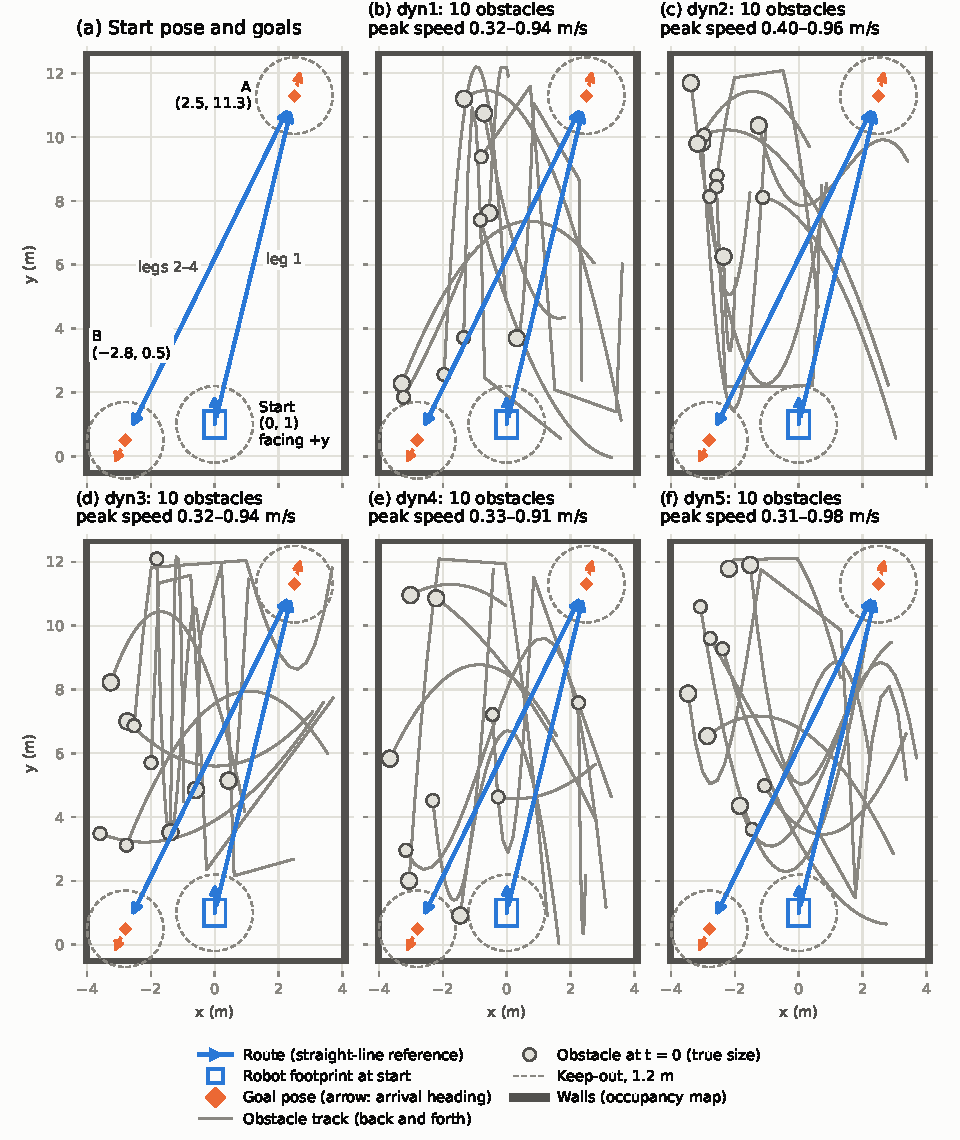
\includegraphics[width=\columnwidth]{figures/benchmark_route_dyn.pdf}
  \caption{Benchmark start pose, goal poses and obstacle tracks for
  \texttt{dyn1}--\texttt{dyn5} over the occupancy map used in all trials.}
  \label{fig:route}
\end{figure}

\subsection{Conditions}
The ablation isolates prediction from topology:
\begin{description}
  \item[A] stock Nav2 MPPI (unmodified baseline);
  \item[B] TG-MPPI, full, legacy (unequal) sample split;
  \item[B$'$] TG-MPPI, full, equal sample split;
  \item[D] plain MPPI plus the predicted-obstacle critic, topology disabled.
\end{description}
Condition D is the critical control: it carries the obstacle prediction but none
of the topological machinery, so the difference $B - D$ measures what topology
contributes over prediction alone.

\subsection{Protocol and metrics}
Every trial starts from a fixed simulation time so that all conditions encounter
identical obstacle phases; goals are issued in a fixed sequence with no
preemption. Contacts are scored from ground truth (robot footprint against
obstacle discs) rather than from the costmap, so a condition cannot score well
by failing to perceive an obstacle. Each condition is run
$5~\text{scenarios} \times 3~\text{repetitions} = 15$ trials, four goal legs
each.
Continuous per-trial metrics are compared with two-sided Mann--Whitney $U$
tests and binary outcome counts with two-sided Fisher exact tests. Statistical
significance is assessed at $\alpha=0.05$ without treating repeated controller
cycles as independent observations. In addition to success, the report records
effective speed, driven-path ratio, minimum clearance, first-contact cause,
recovery count, controller cycle time and deadline misses. Unattempted legs
after early trial termination count as failures in planned-leg success rates.

\subsection{Reference-sandbox protocol}
Before Nav2 integration, the proposed sampling mechanism was frozen and tested
in the independent PyTorch sandbox with the analytical SLIP model. Four
controllers used identical dynamics, footprint, cost weights, limits,
$N=1024$ samples and a 56-step horizon: ordinary MPPI; path-tracking MPPI,
which adds an A* reference only to the rollout cost; single-path Biased MPPI,
which samples around one A*-derived ancillary mean; and full TG-MPPI, which
adds up to three pseudopod-derived ancillary distributions. The ordinary
narrow-navigation matrix comprised ten declared BARN worlds and five matched
sampling seeds (50 runs per controller).

A separate blocked-path experiment isolated the thesis mechanism. It compared
full TG-MPPI against a \emph{flow-only} control with the same geodesic
field, path bias, gate, dynamics and costs, but with pseudopod extraction and
grouped ancillary proposals disabled. Ten paired seeds were used. Outcomes
were compared with an exact two-sided McNemar test. Finally, controller update
time was measured serially on worlds 7, 48 and 42; these Python timings
characterise the reference implementation and are not Nav2 real-time results.

\subsection{Physical SLIP validation plan}
Following the simulation benchmark, a limited matched validation is planned on
the physical SLIP platform. Localisation will be supplied by Vicon and obstacle
observations by the onboard lidar pipeline rather than Gazebo ground truth.
The objective is transfer validation---whether the controller runs at its
required rate and preserves the simulation safety trend under real skid,
latency and sensing---not retraining or retuning on the test course.

Trials will progress from an empty-path check to a static narrow passage and
then to a controlled moving-obstacle crossing. Stock Nav2 MPPI (A), prediction
only (D), and the selected TG-MPPI configuration (B or B$'$) should receive the
same start, goal, speed limit and obstacle script, with controller order
counterbalanced across repetitions. Recorded ROS bags should include Vicon
pose, raw and filtered scans, odometry, velocity commands, global and local
plans, costmaps, tracked-obstacle states, controller diagnostics and TF. The
primary hardware outcomes are goal completion without intervention, minimum
Vicon-based clearance, traversal time, path length, emergency stops and
control-cycle latency. A human-operated emergency stop, conservative initial
speed and a non-human soft obstacle are required for the moving trial.

\section{Results}
\label{sec:results}

\subsection{Reference-sandbox results}
The frozen static matrix establishes the behaviour of the complete method over
the declared development worlds (Table~\ref{tab:sandbox-static}). Full TG-MPPI
MPPI succeeded in all 50 runs with no collision, compared with 45/50 for the
single-path Biased MPPI baseline, 39/50 for path-tracking MPPI and 25/50 for
ordinary MPPI. Exact-footprint revalidation produced zero outcome changes in
all 200 matched runs. These results must not, however, be used alone to claim a
pseudopod effect: although branches were available in 70.9\,\% of TG-MPPI
cycles, a branch was selected in 0\,\% of cycles in this ordinary static
matrix. They support the complete gated controller, while the blocked-path
ablation below supplies mechanism attribution.

\begin{table}[t]
\centering
\caption{PyTorch sandbox static matrix: 10 BARN worlds, five matched seeds per
world. Clearance is averaged over successful runs.}
\label{tab:sandbox-static}
\begin{tabular}{lrrr}
\toprule
Method & Success & Collisions & Clearance (m) \\
\midrule
Vanilla MPPI       & 25/50 & 25 & 0.216 \\
Path-tracking MPPI & 39/50 & 11 & 0.233 \\
Single-path biased & 45/50 &  5 & 0.251 \\
Full TG-MPPI        & 50/50 &  0 & 0.258 \\
\bottomrule
\end{tabular}
\end{table}

\begin{figure}[t]
  \centering
  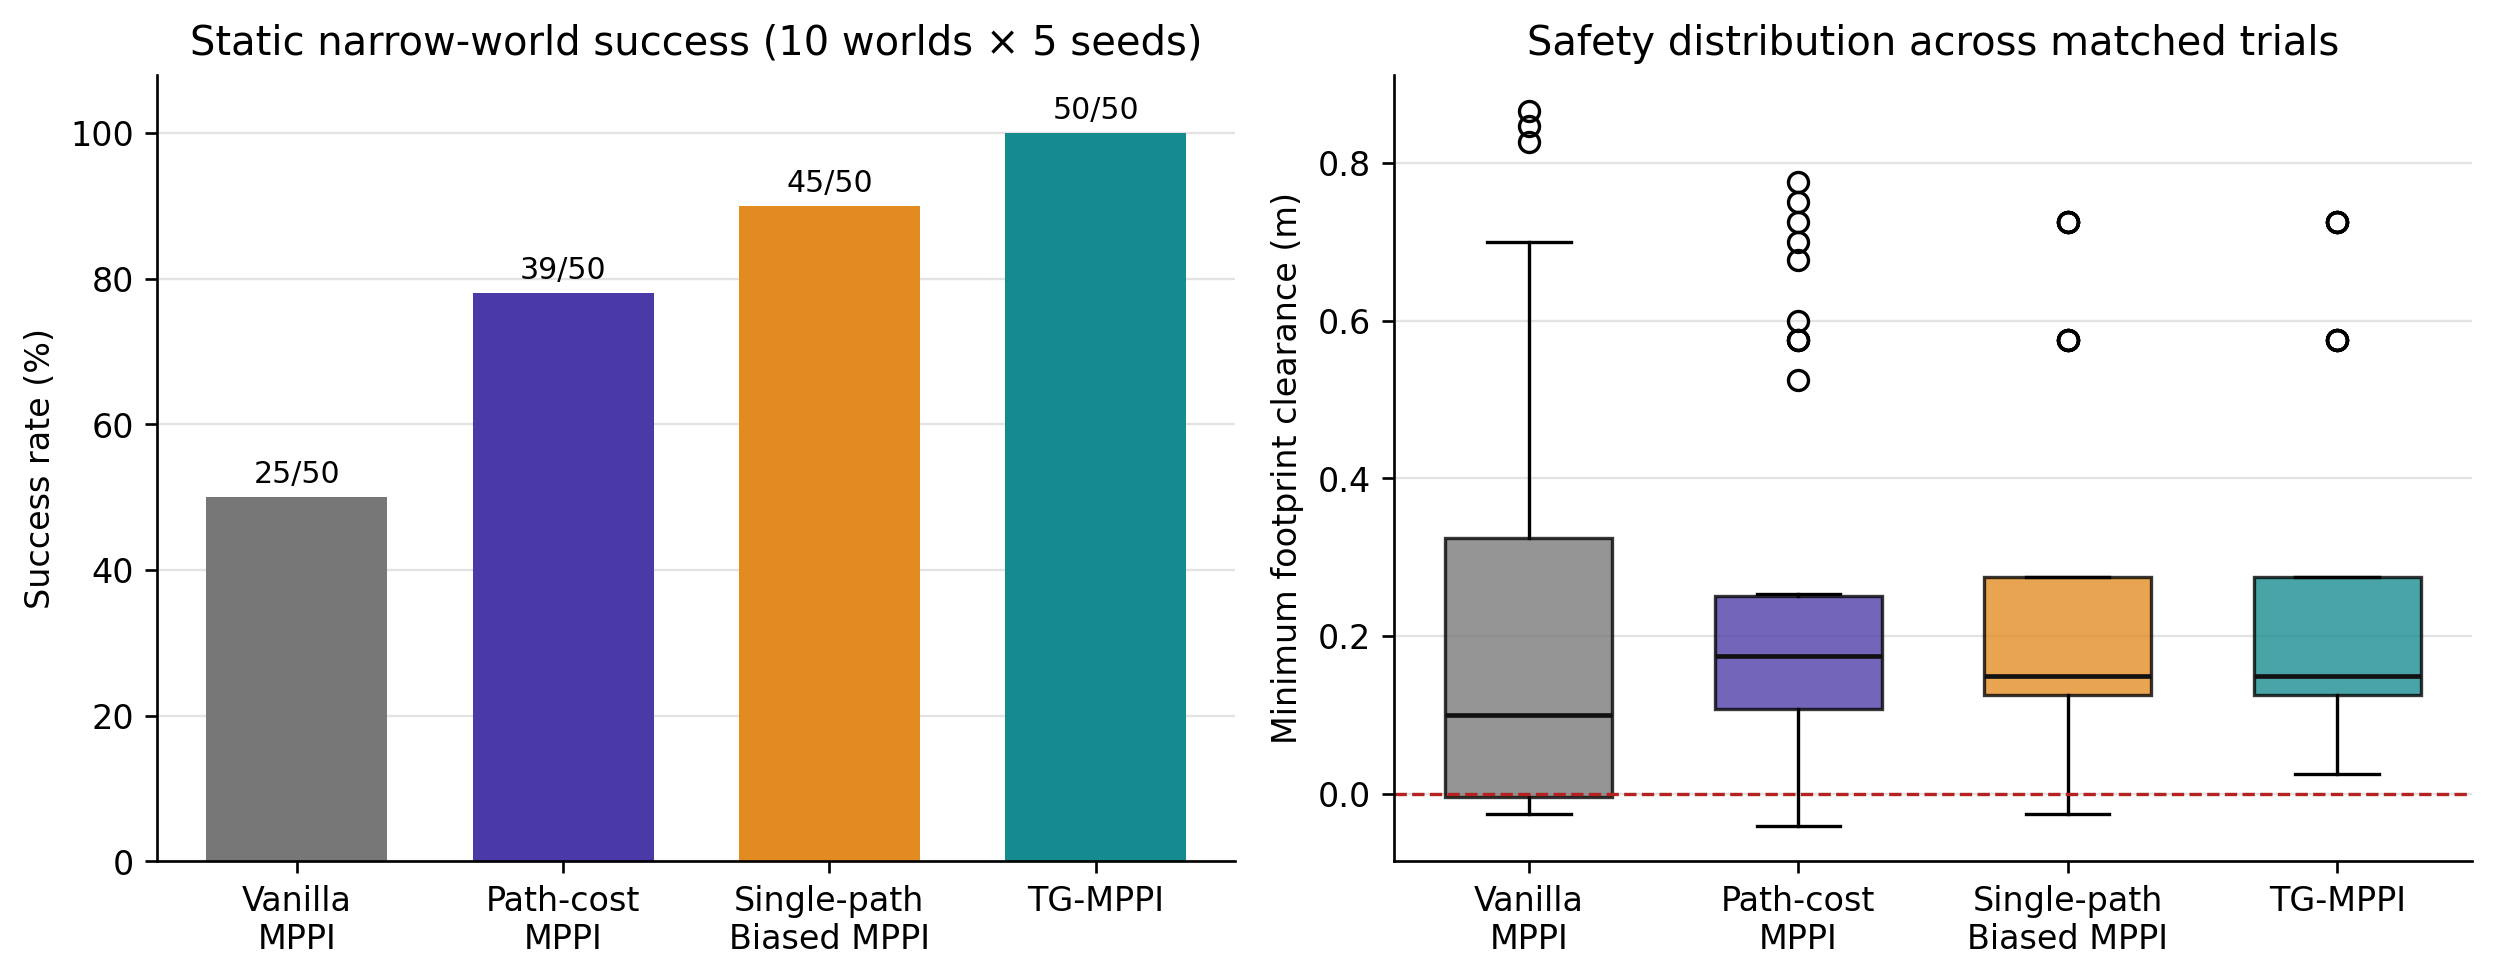
\includegraphics[width=\columnwidth]{../../artifacts/images/experiments/final/static_success_clearance.png}
  \caption{Success and clearance in the frozen sandbox static matrix. This is
  analytical-SLIP reference evidence, not a Gazebo/Nav2 result.}
  \label{fig:sandbox-static}
\end{figure}

The paired blocked-path ablation activated the proposed mechanism
(Table~\ref{tab:sandbox-blocked}). Full TG-MPPI succeeded in 9/10 seeds versus
2/10 for flow-only. There were seven TG-MPPI-only successes, no flow-only-only
successes, two joint successes and one joint failure, giving an exact
two-sided McNemar $p=0.015625$. Pseudopod modes were selected in 47.6\,\% of
TG-MPPI cycles, accompanied by greater peer and static clearance and much less
stall time. This supports a causal contribution from ancillary pseudopod
sampling in the declared deterministic blocked geometry; it does not establish
the same effect across independent environments.

\begin{table}[t]
\centering
\caption{Paired sandbox blocked-path attribution over ten seeds.}
\label{tab:sandbox-blocked}
\begin{tabular}{lrr}
\toprule
Metric & Flow-only & Full TG-MPPI \\
\midrule
Success & 2/10 & 9/10 \\
Peer collisions & 1 & 0 \\
Static collisions & 2 & 0 \\
Timeouts & 5 & 1 \\
Peer clearance (m) & 0.131 & 0.703 \\
Static clearance (m) & 0.028 & 0.143 \\
Mean stall time (s) & 19.96 & 5.02 \\
Pseudopod selection & 0\,\% & 47.6\,\% \\
\bottomrule
\end{tabular}
\end{table}

\begin{figure}[t]
  \centering
  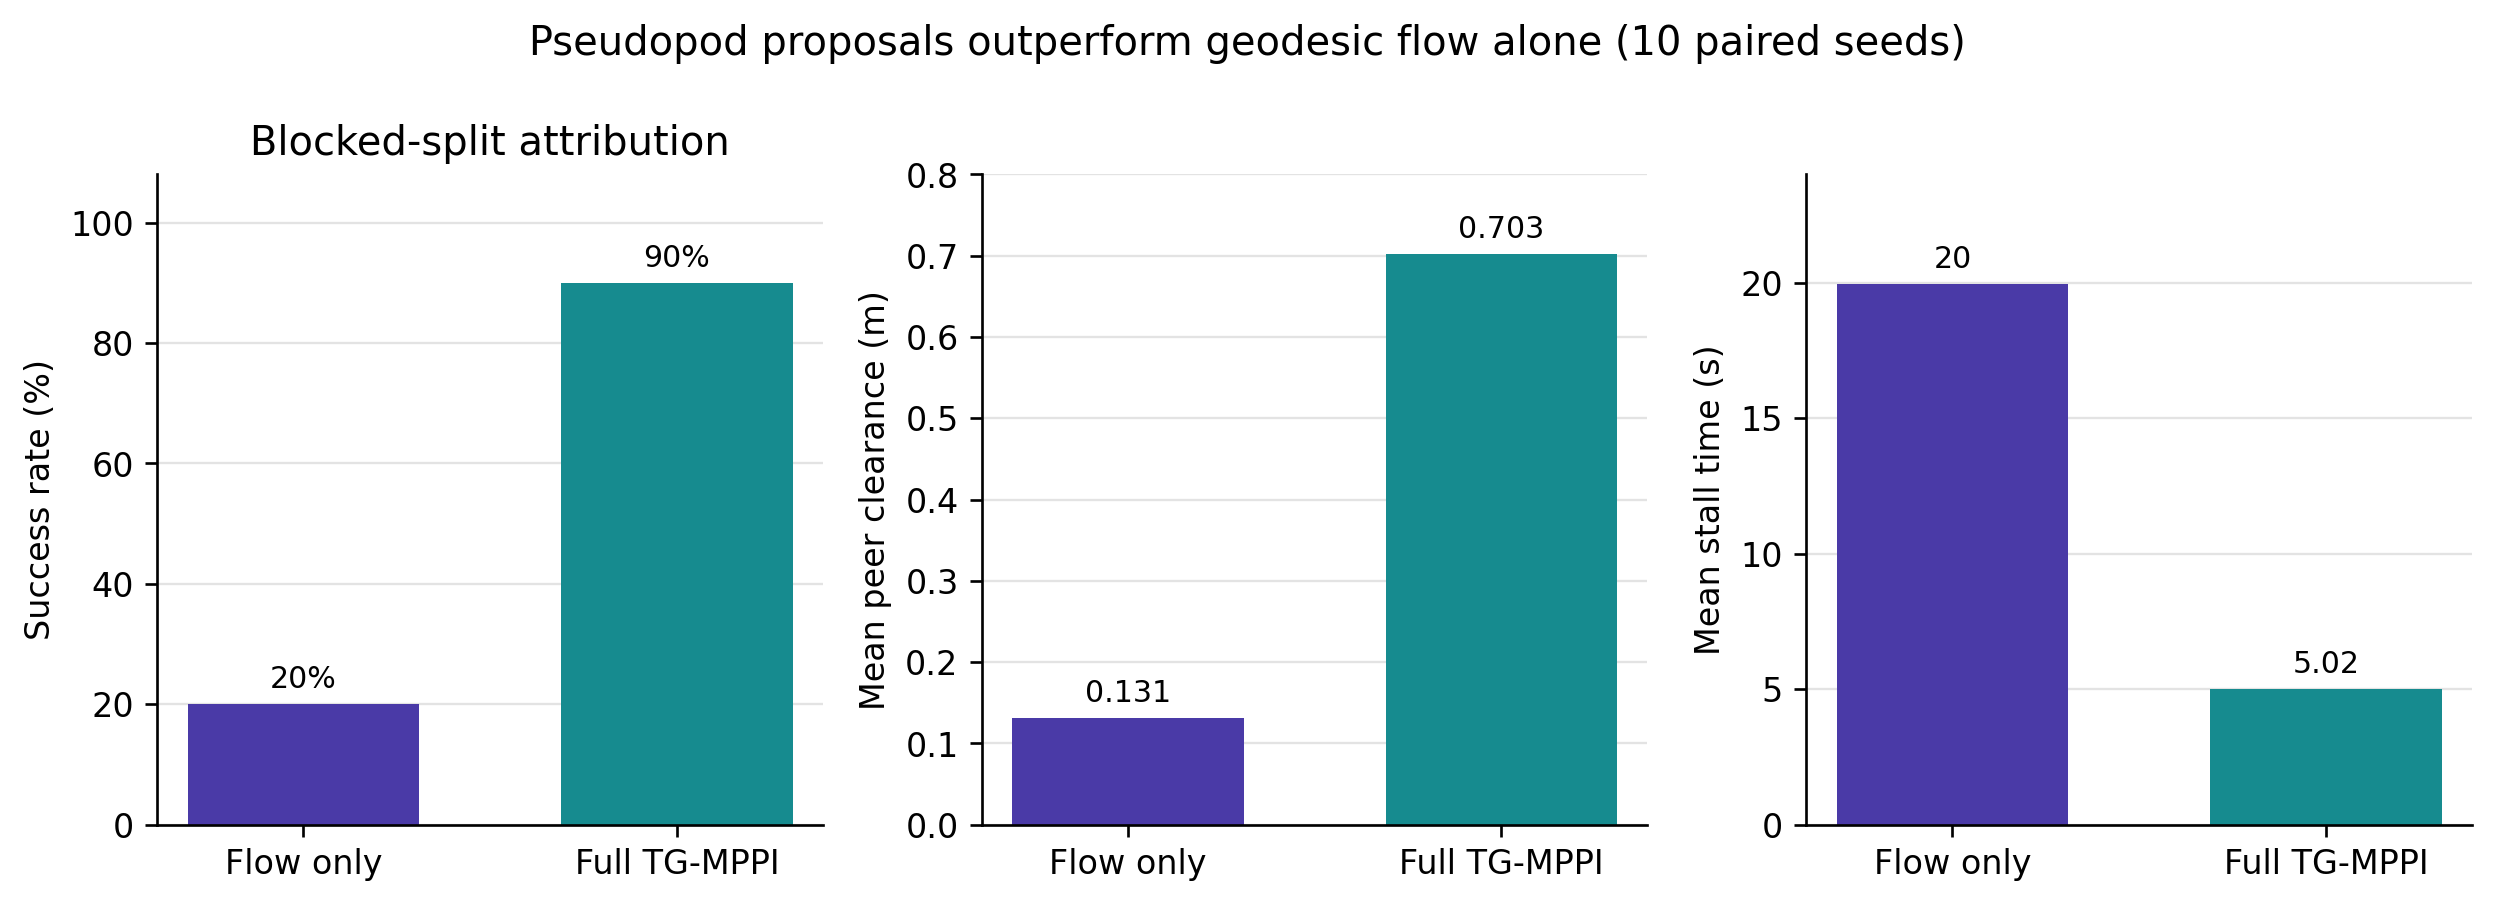
\includegraphics[width=\columnwidth]{../../artifacts/images/experiments/final/blocked_attribution.png}
  \caption{Blocked-path sandbox ablation. Disabling pseudopod proposals while
  retaining geodesic flow sharply reduced completion and clearance.}
  \label{fig:sandbox-blocked}
\end{figure}

Isolated serial timing was 31.45, 109.60, 133.80 and
\SI{147.97}{\milli\second} per update for vanilla, path-tracking,
single-path-biased and full TG-MPPI, respectively. Thus the unoptimised
Python reference does not satisfy a \SI{20}{Hz} budget; TG-MPPI added
\SI{14.17}{\milli\second} (10.6\,\%) over the closest single-path-biased
baseline. This measurement motivated the C++/LibTorch Nav2 implementation and
must not be confused with its measured callback time.

The positive sandbox mechanism result and the Nav2 null topology result below
are not contradictory. The former deliberately blocks the nominal reference
and frequently activates pseudopod proposals; the latter asks whether topology
adds value beyond prediction in five moving-obstacle Gazebo scenarios, where
the corrected measurements did not show such an outcome advantage.

\subsection{Nav2/Gazebo dynamic benchmark}

\begin{table*}[t]
\centering
\caption{Corrected-winding dynamic benchmark: 60 trials (15 per condition,
four planned legs each). Legs ok uses all 60 planned legs per condition;
contacts and continuous metrics use attempted legs because a trial stops after
two consecutive failures. Values are mean $\pm$ standard deviation.}
\label{tab:main}
\begin{tabular}{llcccccc}
\toprule
 & Description & Legs ok & Eff.\ speed (\si{\metre\per\second}) & Legs w/ contact & Min clearance (\si{\metre}) & Recoveries/leg & Cycle (\si{\milli\second}) \\
\midrule
A   & Stock Nav2 MPPI            & 17/60 & $0.83 \pm 0.23$ & 28/44 & $\phantom{-}0.283 \pm 1.491$ & $9.20 \pm 8.10$ & --- \\
B   & TG-MPPI, legacy split      & 54/60 & $0.72 \pm 0.20$ & 13/58 & $\phantom{-}0.246 \pm 0.292$ & $1.29 \pm 3.82$ & $20.0 \pm 0.9$ \\
B$'$& TG-MPPI, equal split       & 52/60 & $0.72 \pm 0.18$ & 14/58 & $\phantom{-}0.211 \pm 0.294$ & $1.71 \pm 4.83$ & $20.1 \pm 1.0$ \\
D   & Plain MPPI + prediction    & 53/60 & $0.71 \pm 0.19$ & \phantom{0}9/57 & $\phantom{-}0.279 \pm 0.286$ & $1.32 \pm 4.47$ & $15.7 \pm 0.5$ \\
\bottomrule
\end{tabular}
\end{table*}

\subsubsection{Prediction accounts for the gain over the baseline}
Table~\ref{tab:main} shows a large and unambiguous separation between the stock
baseline and every condition carrying obstacle prediction. The baseline
completed 17/60 planned legs, compared with 54/60 for B and 53/60 for D.
On per-trial success fraction, A differed from B ($p=6.6\times10^{-5}$) and D
($p=1.2\times10^{-4}$, two-sided Mann--Whitney tests). Treating planned legs as
binary outcomes gives $p=3.1\times10^{-12}$ and
$p=1.7\times10^{-11}$, respectively (Fisher exact tests). Trial-minimum
clearance also improved from A to B ($p=0.007$) and D ($p=0.008$), and
recoveries per planned leg fell in both comparisons ($p<0.001$). Contact in at
least one leg occurred in 14/15 A trials, 10/15 B trials and 8/15 D trials; the
A--D contrast was significant ($p=0.035$), whereas A--B was not ($p=0.169$).
The prediction-only control therefore reproduces the dominant success and
recovery gain over stock MPPI.

\subsubsection{Topology does not separate from prediction}
Under the corrected winding classifier, B completed one more planned leg than
D (54/60 versus 53/60). The per-trial success-fraction difference was
1.7 percentage points (cluster-bootstrap 95\,\% interval
$[-18.3,23.3]$ points; $p=1.0$), and the planned-leg Fisher test also gave
$p=1.0$. Differences in effective speed
($-0.004\,\mathrm{m\,s^{-1}}$, 95\,\% interval $[-0.084,0.076]$,
$p=0.696$), trial-minimum clearance ($-0.013\,\mathrm{m}$,
$[-0.203,0.180]$, $p=0.917$) and recoveries per planned leg (difference
$0.00$, $[-1.95,1.80]$, $p=0.696$) were likewise unresolved. B had contact in
10/15 trials versus 8/15 for D ($p=0.710$).

The measurable difference was computation: B required
\SI{19.99}{\milli\second} per cycle versus \SI{15.71}{\milli\second} for D,
an overhead of \SI{4.28}{\milli\second} (95\,\% interval
$[3.76,4.78]\,\mathrm{ms}$; $p=3.4\times10^{-6}$). Equal allocation B$'$ also
failed to separate from D (52/60 versus 53/60 planned legs, $p=1.0$) and from B
($p=0.777$). The experiment therefore supports a null topology result at this
sample size: it rules out neither modest benefit nor harm, but it provides no
positive evidence that the added modes improve navigation in these scenes.

\subsubsection{Space-time distinctness}
\label{sec:distinctness}
Across the 15 B trials, the space--time gate detected \num{12341} predicted
crossings. The winding test classified \num{794} route pairs (6.4\,\%) as
distinct and \num{11547} as non-distinct. For B$'$, the corresponding counts
were \num{918}/\num{12396} (7.4\,\%) distinct. Controller logs recorded 14 and
17 switches into space--time mode identifiers for B and B$'$, respectively.
These are switch events, not dwell-cycle counts, and should not be interpreted
as a percentage of control authority.

The corrected classifier therefore demonstrates that the space--time layer did
occasionally generate and select distinct alternatives. Nevertheless, neither
B nor B$'$ outperformed D. The earlier 96.7\,\% ``non-distinct'' figure is not
used as evidence of route redundancy: it was produced by the obsolete
synchronised-time test, which was structurally blind to routes passing the same
moving obstacle at different time indices. The corrected experiment changes
the diagnostic interpretation but not the benchmark conclusion.

\subsubsection{Space-time blob and obstacle density}
\label{sec:blob-density}
The space--time layer in Table~\ref{tab:main} only ever proposes up to two
extra modes when a single pseudopod detects a predicted crossing. A further
question is whether a genuine \emph{time-expanded} geodesic body --
flooding $(x,y,t)$ directly, with every predicted obstacle at once, instead
of a per-branch triggered search -- changes the conclusion, and whether that
conclusion holds as obstacle density rises. We implemented this extension
(\emph{the space--time blob}) in both the reference sandbox and the Nav2
port: the local body, membrane and pseudopods of
Section~\ref{sec:method-distinct} are re-derived over a light-cone grid
$(2K{+}1)^2$ cells, $K=\lceil T_{\mathrm{h}}/\Delta t_\ell\rceil$, with one
cell of motion permitted per time layer and free\-/blocked evaluated against
every tracked obstacle's constant-velocity prediction
(Eq.~\ref{eq:cv-prediction}) simultaneously. Candidate exits on the final
layer are ranked by space--time cost plus the static water level as a
terminal cost-to-go, and pseudopods are chosen by homotopy class
(Eq.~\ref{eq:winding}) before falling back to spatial separation. Two
integration modes were evaluated: adding up to two extra proposals in the
same way as the triggered search (\emph{blob-extras}), and replacing the
three ordinary pseudopod slots with the blob's own routes while a hysteresis
gate judges the obstacles to matter (\emph{blob-pods}). Both are gated off
by default and add no measurable cost when inactive ($<2\,\mathrm{ms}$ build
time when active).

To test density, three additional five-obstacle scenes from
Section~\ref{sec:setup} were extended to 15 and 20 obstacles
using the same generator and constraints (Section~\ref{sec:setup}),
giving matched scenes that differ only in obstacle count. Table~\ref{tab:blob}
reports legs completed and legs with contact for B (unmodified TG-MPPI),
blob-extras, blob-pods, and a GPU-backend twin of B, at 10, 15 and 20
obstacles (2 repetitions per world; this is a smaller, exploratory run and
p-values should be read as indicative, not as a powered test).

\begin{table}[t]
\centering
\caption{Legs completed by obstacle density (10/15/20 obstacles), space-time
blob variants. B is unmodified TG-MPPI (Table~\ref{tab:main}); B$_{\mathrm
g}$ is B on the CUDA backend; blob-extras and blob-pods are the two
space-time-blob integration modes.}
\label{tab:blob}
\begin{tabular}{lccc}
\toprule
Condition & 10 obstacles & 15 obstacles & 20 obstacles \\
\midrule
B              & 24/24 (100\%) & 10/14 (71\%) & 11/14 (79\%) \\
B$_{\mathrm g}$& 24/24 (100\%) & 13/15 (87\%) & \phantom{0}7/12 (58\%) \\
Blob-extras    & 23/24 (96\%)  & \phantom{0}8/14 (57\%) & \phantom{0}5/12 (42\%) \\
Blob-pods      & 24/24 (100\%) & 12/15 (80\%) & \phantom{0}3/11 (27\%) \\
\bottomrule
\end{tabular}
\end{table}

\begin{figure*}[t]
  \centering
  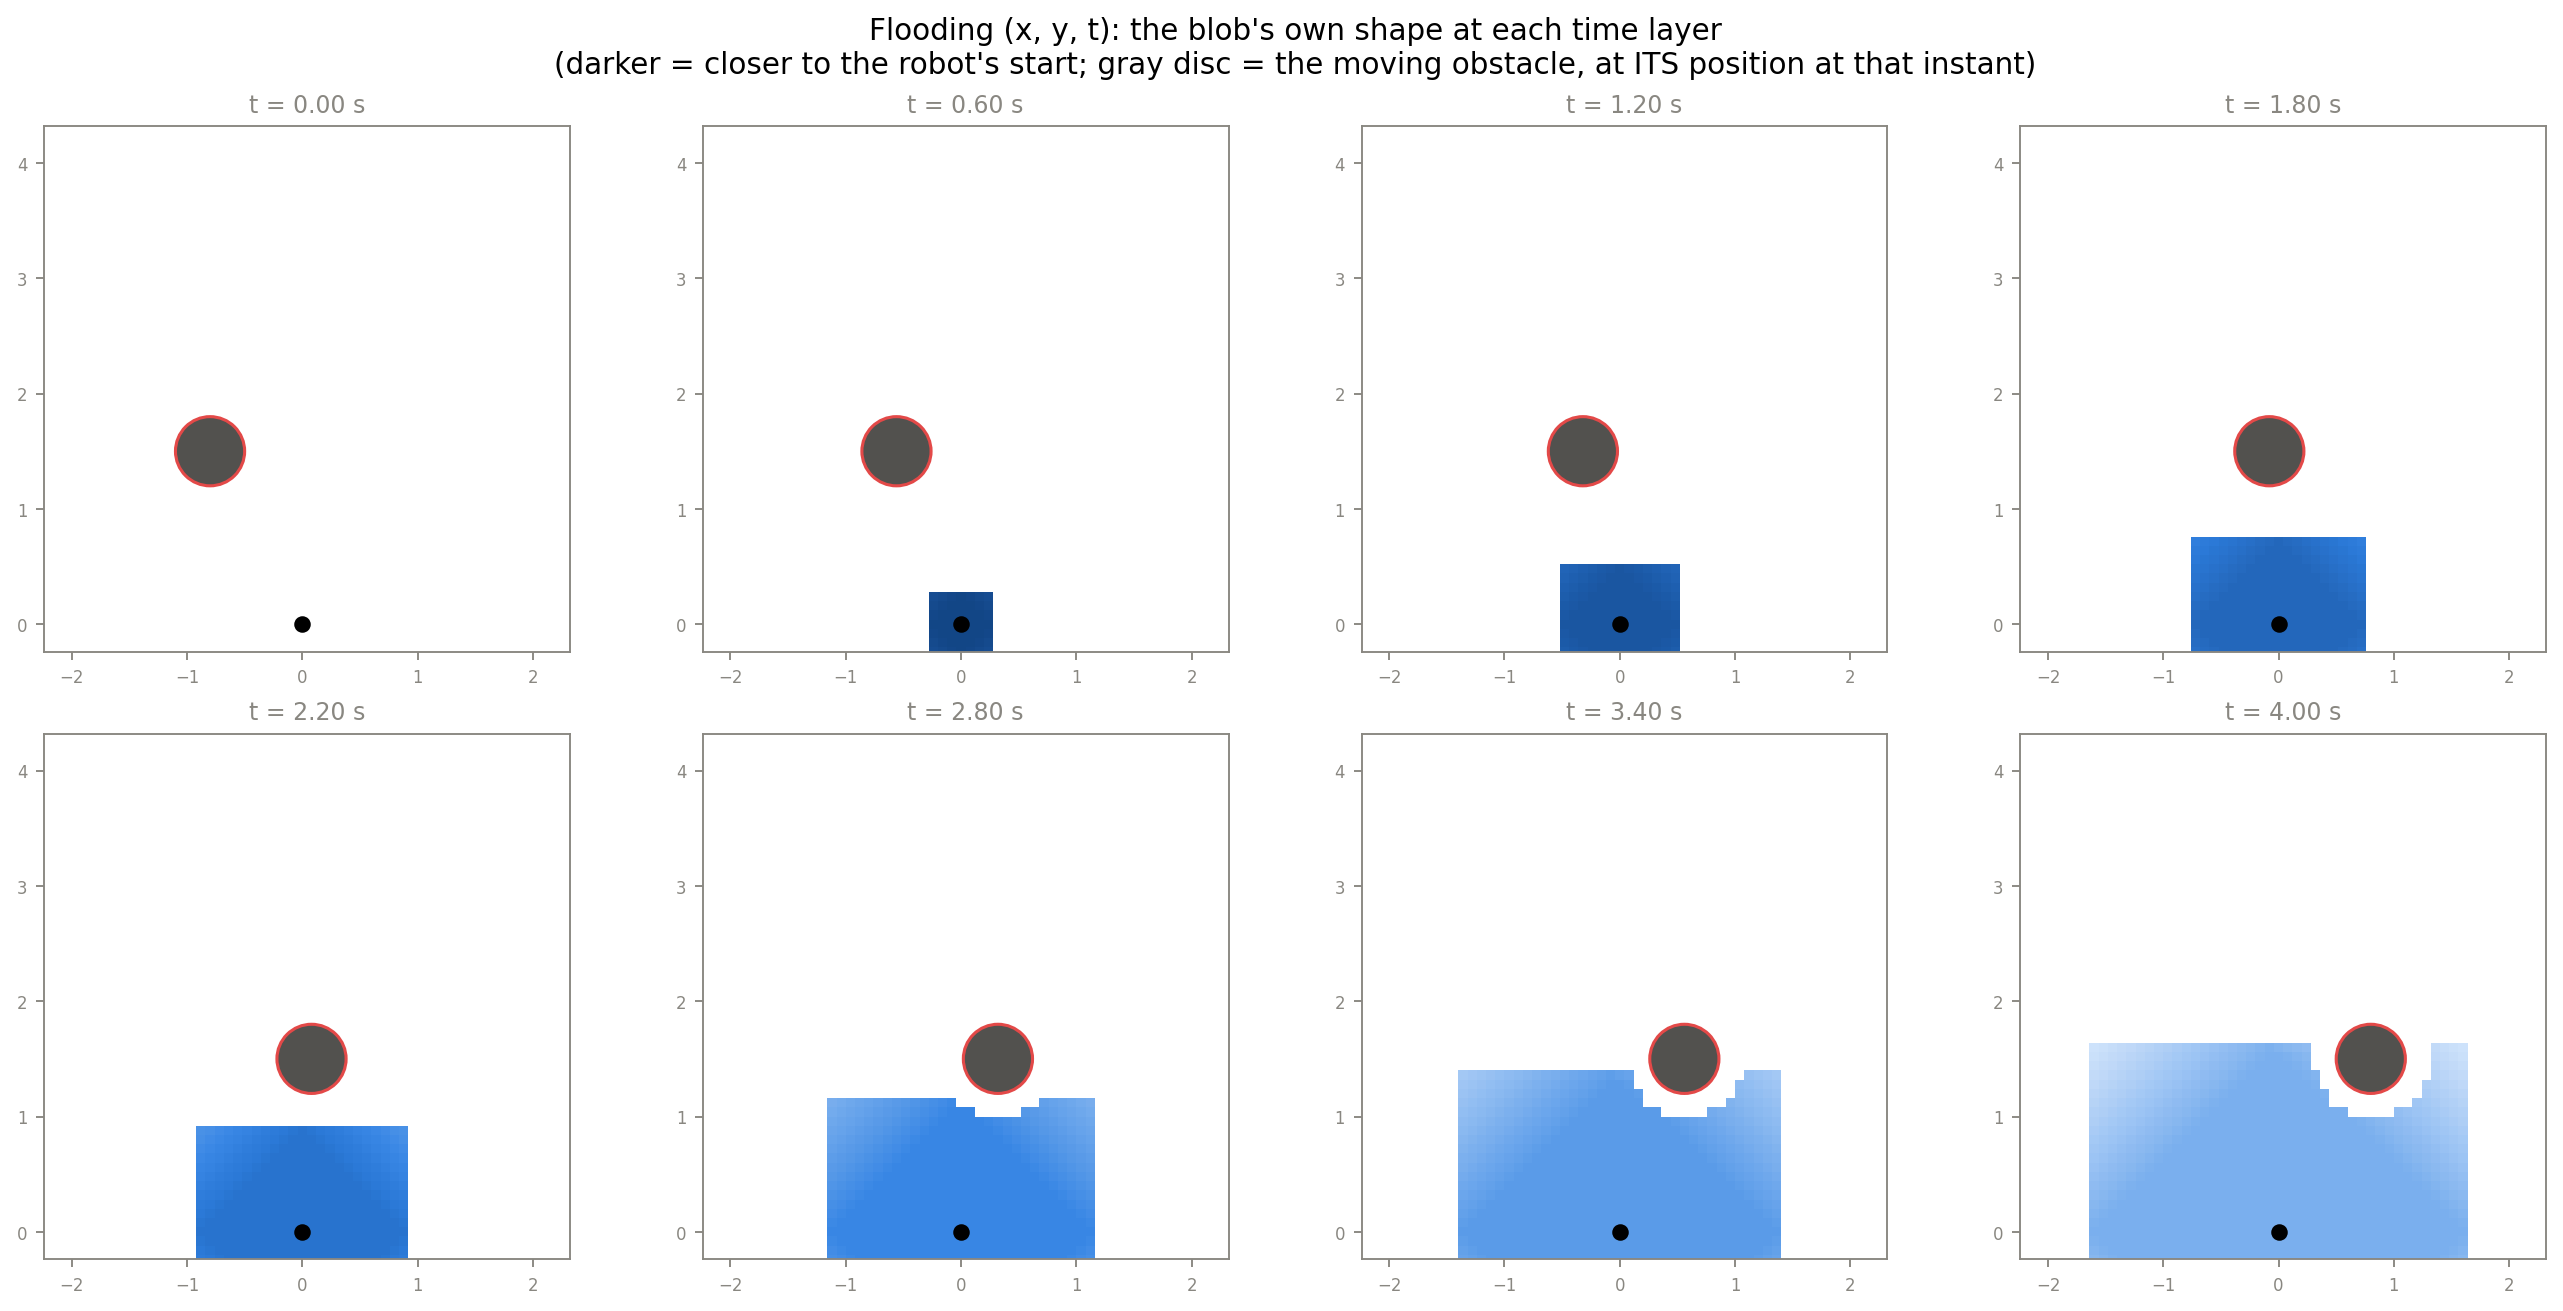
\includegraphics[width=0.92\textwidth]{figures/spacetime_flood_filmstrip.png}
  \caption{The mechanism the space--time blob generalises: flooding $(x,y,t)$
  keeps the full reachable set at every time layer, not just two candidate
  routes through it (reference-sandbox prototype, single synthetic obstacle,
  \SI{4}{\second} horizon, \SI{0.2}{\second} layers). The reachable region
  grows from the robot's start (darker = fewer layers elapsed) and is bitten
  into by the obstacle's own moving footprint (gray disc) as the flood
  advances -- the same notch that separates the wait and detour homotopy
  classes extracted by \texttt{SpaceTimeBody} (Section~\ref{sec:blob-density}).
  Shown for intuition; the quantitative claims of
  Section~\ref{sec:blob-density} come only from the matched Gazebo and
  sandbox panels.}
  \label{fig:spacetime-flood-mechanism}
\end{figure*}

\begin{figure}[t]
  \centering
  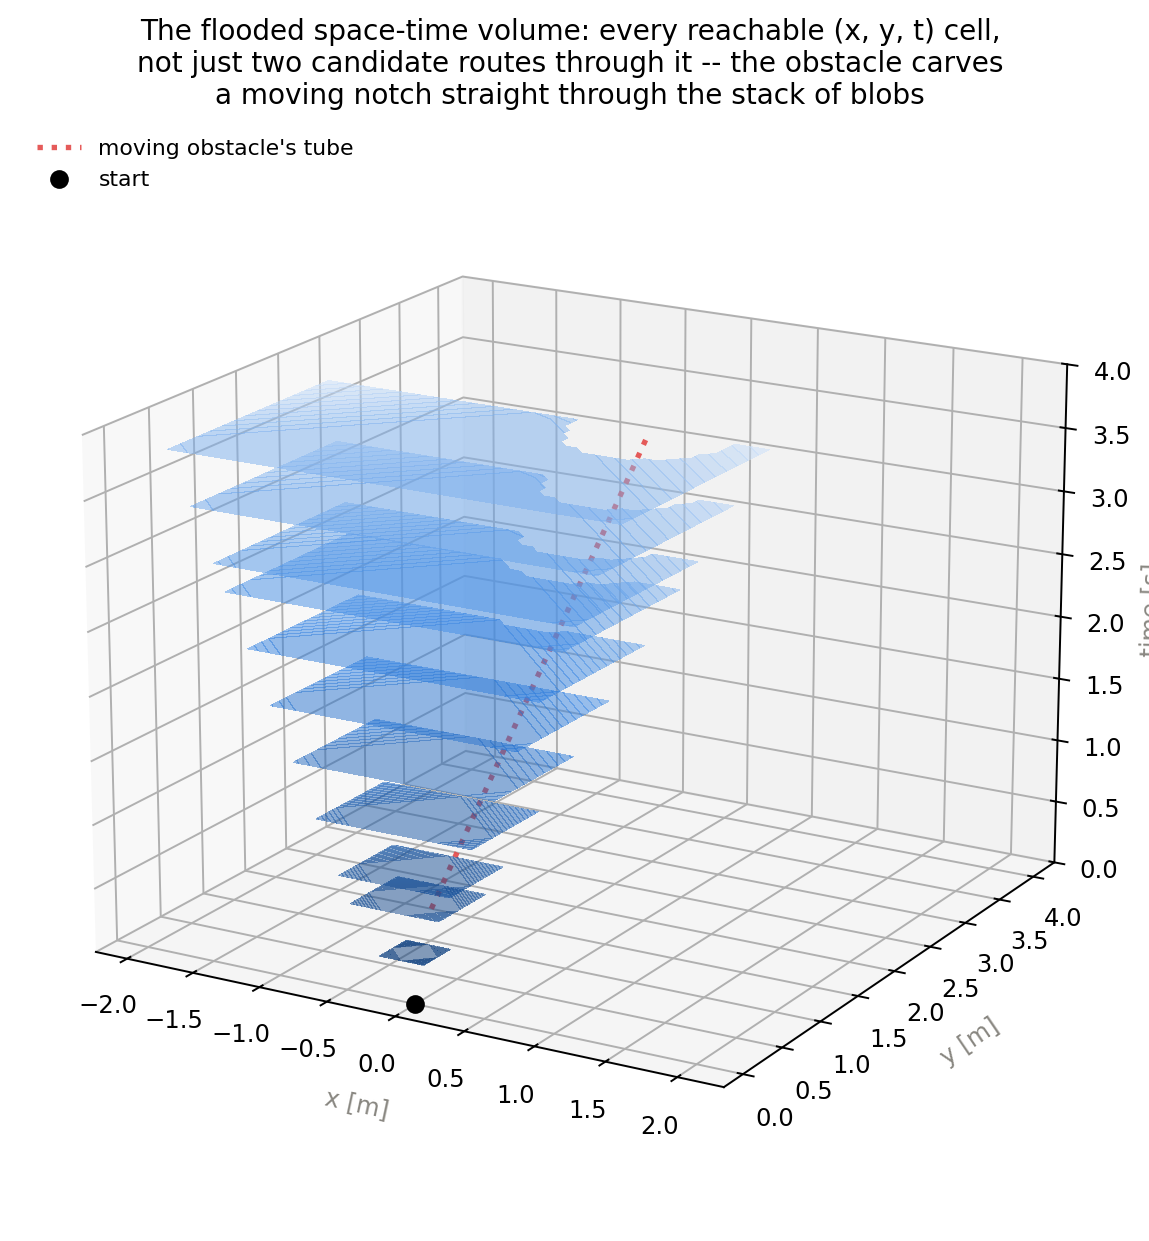
\includegraphics[width=\columnwidth]{figures/spacetime_flood_volume.png}
  \caption{The same flood as a stack of time layers in $(x,y,t)$. Each
  translucent sheet is one layer's reachable set (Fig.~\ref{fig:spacetime-flood-mechanism}
  collapsed to a single instant); the dotted line is the moving obstacle's
  own trajectory traced through time, i.e.\ the exclusion tube each layer's
  notch is a cross-section of. A route that stays on one side of the tube
  throughout is one homotopy class; a route that crosses to the other side
  is distinct under Eq.~\ref{eq:winding}.}
  \label{fig:spacetime-flood-volume}
\end{figure}

At 10 obstacles every condition matches or is within one leg of B, consistent
with Table~\ref{tab:main}: the blob changes nothing when the scene is easy.
As density rises, both blob variants fall further behind B rather than
closing the gap, and blob-pods -- the mode that most changes the sampling
distribution -- degrades fastest, from matching B at 15 obstacles to the
worst result of any condition at 20 (27\% legs completed, 64\% of legs with
at least one contact, $9.3$ recoveries per leg). Paired against B leg-by-leg
on the dense scenes, none of the three variants differs from B beyond what
this sample size can resolve (McNemar exact, blob-extras $p=0.39$, blob-pods
$p=0.55$, B$_{\mathrm g}$ $p=1.0$), but the direction is consistent with an
independent reference-sandbox panel (240 episodes, N$\in\{10,20,30\}$ random
waypoint-moving obstacles, 20 seeds per cell), where the blob likewise
tracked the existing wait/detour mechanism rather than improving on it
(pooled $N{\ge}20$: base 27/40, blob-pods 30/40, $p=0.45$). We therefore do
not adopt the space--time blob: across four independent tests -- the sandbox
panel, two single-scene Gazebo probes, and this density sweep -- it never
separates from the existing method, and in the one setting it changes the
most (dense scenes with the pseudopod slots replaced) it is measurably worse.
It is reported here as an implemented and evaluated negative result rather
than included in the method under test.

The CUDA backend (B$_{\mathrm g}$) shows no consistent advantage either: mean
cycle time was \SI{21.1}{\milli\second}, statistically indistinguishable from
B's CPU cycle time in this run, because trajectory noise generation and the
softmax weighting update remain CPU-bound in the current port and the
predicted-obstacle critic is CPU-only under both backends. GPU offload
therefore accelerates the critics it covers without yet changing wall-clock
behaviour end to end; a port of the remaining CPU stages is future work.

\section{Discussion and Limitations}
\label{sec:discussion}
The ablation is designed to prevent a useful prediction mechanism from being
mistaken for evidence of topological reasoning: condition D receives the same
predicted-obstacle critic as TG-MPPI but no pseudopod or space--time proposal.
Topology is therefore assessed from B versus D in the corrected winding-test
run, not from TG-MPPI versus the stock baseline. That comparison is a null
result: the observed 1.7-point success difference is negligible relative to its
wide $[-18.3,23.3]$-point interval, while the computational overhead is clear.
This is not proof that topology can never help. Resolving a modest effect would
require more repetitions and scenes deliberately containing two feasible
classes with different temporal consequences; the present five scenarios do
not provide that evidence.

Scenario coverage is limited to five scripted obstacle patterns over one map.
Although restarting Gazebo and fixing the first-goal simulation time makes
conditions comparable, it does not establish generality across building
layouts, crowd densities or obstacle behaviours. In particular, the obstacles
follow known polynomial tracks, whereas the controller observes position and
velocity and extrapolates constant velocity. Abrupt acceleration or reversal
therefore produces prediction error. The reported trials also use perfect
ground-truth obstacle observations without perception noise, delay, missed
detections or identity switches. The available tracking-quality perturbations
and a real lidar tracker remain validation work rather than evidence included
in the main result.

The main controlled experiment is simulation-only. Gazebo contact and skid
behaviour cannot substitute for hardware tests of wheel slip, actuator delay
and safety stops; the planned physical trials are therefore reported as a
separate transfer study and must not be described as completed until their bags
have been scored.
Furthermore, the winding classifier is a pragmatic finite-route test rather
than a complete topological invariant for every local geometry. A route that
passes far from an obstacle can accumulate less than the $1/(4\pi)$ pass
threshold and be classified as not having passed it. This failure mode should
be reported alongside the corrected distinctness rate.

\section{Conclusion}
This thesis presented TG-MPPI, a Nav2 controller that turns a robot-centred
geodesic flood field into collision-validated ancillary MPPI proposals and can
augment them with time-expanded wait/detour routes. A reproducible Gazebo
benchmark compares it with an untouched stock Nav2 MPPI controller and, through
a prediction-only condition, separates obstacle prediction from topology.
TG-MPPI completed 54/60 planned dynamic-obstacle legs compared with 17/60 for
stock MPPI, but prediction-only MPPI completed 53/60. With winding-based route
classification, TG-MPPI remained statistically indistinguishable from the
prediction-only control on success, clearance and speed while costing an
additional \SI{4.28}{\milli\second} per cycle. The defensible conclusion is
therefore that predicted-obstacle handling explains the measured improvement;
the topological proposal layer is implemented and occasionally active, but its
navigation benefit was not demonstrated by this benchmark.
The result should be interpreted within the limits of perfect obstacle
tracking, five simulated scenarios and no physical-robot validation.

\section*{Acknowledgment}
The author thanks his supervisor, Dr.\ Laura Ferranti (R2C Lab, Delft
University of Technology, e-mail: L.Ferranti@tudelft.nl), for her guidance
throughout this project.

\bibliographystyle{IEEEtran}
\bibliography{refs}

\end{document}
